\section{Results}
In this section, we assess the performance of LineaMapper v1.1 and v2.0. Then, we analyze the manually revised and fully automatically generated maps.

%% LineaMapper v1.1 on new test set --> 2024_06_15_10_54_26_metricsdict_bbox_v2_112_comparison.csv
\begin{table*}%[htbp!]
\centering
\caption{LineaMapper v1.1 and v2.0 bounding box average precision (AP) and average recall (AR), per class and averaged over classes, in percent, for the test dataset shown in \Cref{fig:full_map}.C, tiled to 112x112 pixel tiles. The subsets $0.35$ and $0.50$ stand for an IoU threshold of 0.35 and 0.5, respectively, and $S$, $M$, and $L$ indicate small, medium, and large objects evaluated at an IoU range of 0.50 to 0.95. In contrast, no subset evaluates all object sizes at an IoU range of 0.50 to 0.95.}
\label{tab:bbox_metrics_v1.1_112x112}
\begin{tabular}{@{}lcccccc|cccccc@{}}
\toprule
 & AP$_{0.35}$ & AP$_{0.50}$ & AP & AP$_S$ & AP$_M$ & AP$_L$ & AR$_{0.35}$ & AR$_{0.50}$ & AR & AR$_S$ & AR$_M$ & AR$_L$ \\ \midrule
Bands & 14.1 & 12.3 & 6.0 & 3.1 & 8.2 & 33.0 & 62.8 & 53.5 & 32.1 & 18.6 & 42.2 & 76.0 \\
Double ridges & 45.6 & 44.0 & 25.7 & 16.5 & 36.8 & 66.7 & 83.8 & 82.0 & 49.0 & 40.3 & 59.7 & 70.0 \\
Ridge complexes & 21.3 & 19.6 & 10.5 & 3.1 & 14.6 & 59.1 & 69.1 & 67.9 & 39.3 & 21.3 & 49.0 & 63.3 \\
Undiff. lineae & 26.1 & 25.1 & 12.7 & 11.3 & 17.1 & 50.0 & 71.4 & 69.1 & 38.0 & 33.9 & 48.3 & 50.0 \\ \midrule
Mean & 25.7 & 24.2 & 13.2 & 8.2 & 19.2 & 52.2 & 68.9 & 65.4 & 38.0 & 27.4 & 49.8 & 64.8 \\ \bottomrule
\end{tabular}
\end{table*}


% LineaMapper v1.1 only (mask rcnn) ---> 2024_06_15_15_50_39_metricsdict_segm_run10_onRegmaps112_comparison.csv
\begin{table*}%[htbp!]
\centering
\caption{LineaMapper v1.1, else, same as \Cref{tab:bbox_metrics_v1.1_112x112} for masks.}
\label{tab:segm_metrics_v1.1_112x112}
\begin{tabular}{@{}lcccccc|cccccc@{}}
\toprule
 & AP$_{0.35}$ & AP$_{0.50}$ & AP & AP$_S$ & AP$_M$ & AP$_L$ & AR$_{0.35}$ & AR$_{0.50}$ & AR & AR$_S$ & AR$_M$ & AR$_L$ \\ \midrule
Bands & 9.6 & 8.1 & 2.9 & 1.2 & 4.4 & 24.3 & 45.3 & 40.7 & 16.5 & 11.6 & 21.4 & 24.0 \\
Double ridges & 35.9 & 32.5 & 12.5 & 6.9 & 22.6 & 24.3 & 60.7 & 55.1 & 24.1 & 25.2 & 22.6 & 24.0 \\
Ridge complexes & 16.2 & 12.8 & 4.9 & 0.8 & 8.7 & 20.0 & 55.6 & 50.6 & 23.0 & 17.3 & 26.7 & 20.0 \\
Undiff. lineae & 17.3 & 14.9 & 5.0 & 4.3 & 12.3 & 10.0 & 47.6 & 41.3 & 17.0 & 19.0 & 12.0 & 10.0 \\ \midrule
Mean & 19.0 & 16.4 & 6.1 & 3.2 & 12.0 & 19.6 & 50.2 & 45.0 & 19.3 & 17.5 & 20.7 & 19.5 \\ \bottomrule
\end{tabular}
\end{table*}


% rcnnSAM -- > 2024_06_15_10_54_26_metricsdict_segm_v2_112_comparison.csv
\begin{table*}%[htbp!]
\centering
\caption{For LineaMapper v2.0, else, same as \Cref{tab:segm_metrics_v1.1_112x112}.}
\label{tab:segm_metrics_v2.0_112x112}
\begin{tabular}{@{}lcccccc|cccccc@{}}
\toprule
 & AP$_{0.35}$ & AP$_{0.50}$ & AP & AP$_S$ & AP$_M$ & AP$_L$ & AR$_{0.35}$ & AR$_{0.50}$ & AR & AR$_S$ & AR$_M$ & AR$_L$ \\ \midrule
Bands & 6.6 & 4.2 & 1.3 & 0.4 & 3.1 & 16.4 & 25.6 & 19.8 & 8.1 & 2.5 & 13.8 & 16.0 \\
Double ridges & 30.3 & 25.3 & 9.9 & 4.8 & 18.7 & 34.3 & 49.6 & 42.6 & 19.2 & 18.4 & 19.7 & 34.0 \\
Ridge complexes & 11.7 & 8.4 & 3.3 & 1.1 & 6.6 & 20.0 & 40.7 & 35.8 & 16.7 & 13.0 & 18.8 & 20.0 \\
Undiff. lineae & 9.1 & 6.6 & 2.5 & 1.8 & 7.8 & 0.0 & 32.0 & 24.9 & 11.1 & 12.0 & 8.9 & 0.0 \\ \midrule
Mean & 13.8 & 10.7 & 4.1 & 1.9 & 9.1 & 17.7 & 35.5 & 29.5 & 13.2 & 11.0 & 15.3 & 17.5 \\ \bottomrule
\end{tabular}
\end{table*}


% combined model comparison: ---> combined_model_comparison_smalledit.csv
\begin{table*}%[htbp!]
\centering
\caption{Model comparison of average precision and average recall class average. For an overview of the different models, see \Cref{tab:Model_overviwe}.}
\label{tab:segm_comparison}
\begin{tabular}{@{}lcccccc|cccccc@{}}
\toprule
Model & AP$_{0.35}$ & AP$_{0.50}$ & AP & AP$_S$ & AP$_M$ & AP$_L$ & AR$_{0.35}$ & AR$_{0.50}$ & AR & AR$_S$ & AR$_M$ & AR$_L$ \\ \midrule
LM 2.0 & 13.8 & 10.7 & 4.1 & 1.9 & 9.1 & 17.7 & 35.5 & 29.5 & 13.2 & 11.0 & 15.3 & 17.5 \\
LM 1.1 & 19.0 & 16.4 & 6.1 & 3.2 & 12.0 & 19.6 & 50.2 & 45.0 & 19.3 & 17.5 & 20.7 & 19.5 \\
SAM-pp & 9.7 & 7.4 & 2.9 & 0.6 & 7.3 & 11.8 & 17.0 & 13.8 & 6.1 & 2.8 & 10.2 & 11.7 \\
SAM-GR & 17.2 & 13.6 & 5.1 & 3.5 & 13.7 & 16.9 & 36.7 & 31.5 & 13.8 & 11.9 & 15.7 & 16.7 \\
RCNN-SAM-t & 8.7 & 5.8 & 2.2 & 1.0 & 5.1 & 12.2 & 31.1 & 23.8 & 10.1 & 9.0 & 11.3 & 12.0 \\
SAM-pp-t & 3.6 & 2.5 & 1.0 & 0.5 & 2.1 & 7.6 & 8.2 & 6.1 & 2.5 & 1.7 & 2.9 & 7.5 \\ \bottomrule
\end{tabular}
\end{table*}

\subsection{Improvements of LineaMapper}\label{sec:lineamapper_compar}
% fine tuning for 112x112 pixel tiles
% more complete map, more stable results
% performance metrics (discuss tables)
% describe qualtitative figure comparisons
We discuss improved versions of LineaMapper versions 1.1 and 2.0 by comparing performance metrics. We compare the assembled model predictions to pre-existing maps and the manually revised map.

\subsubsection{Performance of LineaMapper v1.1}\label{sec:LM1.1}
In Tables \ref{tab:prec_rec_iou05} - \ref{tab:segm_metrics_v1.1_112x112}, we present performance metrics of LineaMapper v2.0 on the test dataset (\Cref{fig:full_map}.C).
We find that fine-tuning LineaMapper works best for smaller images of 112x112 pixels, on the one hand, because with a minimum size of 200~px, lineaments are magnified and occupy more pixels than they would in 112~px tiles, and on the other hand, because with the additional training data, the complexity increases compared with the training images in\sidecite{Haslebacher2024a}. First, the increased complexity is linked to the lowered guideline criteria for a lineament to be mapped, and second, the regional resolution of 215 m/px resolves more detail than training data at 500 m/px, which were, amongst others, used for LineaMapper v1.0. Therefore, we compare the performance results of LineaMapper v1.1 directly to the performance achieved by LineaMapper v1.0 on the same test set (\Cref{fig:full_map}.C) in the following. 

% Table precision-recall
LineaMapper v1.1 shows increased recall values for both bounding boxes and masks when compared with LineaMapper v1.0 on the regional test set (\Cref{tab:prec_rec_iou05}). This increase in recall is traded with a decrease in precision, except for undifferentiated lineae, which benefit from more complete mapping due to the adapted guideline as well as the smaller tile size of 112 pixel tiles. In fact, the 112x112 pixel tiles get resampled to 200x200 pixel tiles, which amplifies the size of the lineaments. The average values for recall and precision in \Cref{tab:prec_rec_iou05} are now similar: for bounding boxes, the precision and recall are both 31-32\% and for masks, 25-26\%. This means that, at an IoU of 0.5 and a class score threshold of 0.5 (50\%), the number of false positives (wrong predictions) is similar to the number of false negatives\sidenote{\ie~undetected ---missed --- or only partially predicted lineaments}. When the ground truth (GR) bounding boxes are used to prompt SAM (SAM-GR), the mask precision increases from 25.8\% to 37\%, and the recall increases from 25\% to 27\%.


% Table average precision and average recall tab:bbox_metrics_v1.1_112x112
LineaMapper v1.1 increases its performance by 7.7\% and 4.0\% in average precision (AP) and by 10.7\% and 7.3\% in average recall (AR) for bounding boxes and masks, respectively (\Cref{tab:bbox_metrics_v1.1_112x112,tab:segm_metrics_v1.1_112x112}), when we consider the mean of all categories. The increase in performance is 11 to 17\% for constant IoU-score thresholds of 0.35 and 0.50 (AP$_{0.35}$, AP$_{0.50}$, AR$_{0.35}$, AR$_{0.50}$). The categories that perform best are double ridges, while bands perform worst but are better than v1.0. The difference to LineaMapper v1.0 in performance is the lowest for ridge complexes and bands.
% discussion: interpretation. why might this be? bands: units! too wide for 112x112 for training (not inference)
% compare to LineaMapper v1.0. compare to other test sets.
For photometrically corrected images, the performance decreases slightly for bounding boxes and masks, except for large objects ($AP_L$, $AR_L$), although qualitative results are comparable (not shown). Therefore, we decided to feed the original SSI images instead of photometrically corrected images constituting the RegMaps into LineaMapper.


\subsubsection{Performance of LineaMapper v2.0 (Mask R-CNN + SAM)}\label{sec:LM2.0}
In \Cref{tab:segm_metrics_v2.0_112x112}, we present performance metrics of LineaMapper v2.0 on the test dataset (\Cref{fig:full_map}.C). Since the bounding boxes come from LineaMapper v1.1, we only need to discuss mask performance (\Cref{tab:segm_metrics_v2.0_112x112}) in comparison to v1.1 and v1.0. In comparison to v1.0, the average precision (AP) increases by 2.0\%, while the average recall increases by 1.2\%. % This means that more pixels were missed (more false negatives) while fewer additional pixels are predicted (less false positives). The best performance is reached for double ridges.
The increase in average precision is 6 to 7\% for constant IoU-score thresholds of 0.35 and 0.50 (AP$_{0.35}$, AP$_{0.50}$), and 1\% for average recall (AR$_{0.35}$, AR$_{0.50}$).
The performance of LineaMapper v2.0 is lower than or equal to the Mask R-CNN metrics (\Cref{tab:segm_metrics_v1.1_112x112}) for nearly all ($\approx$90\%) metrics. The average precision of large objects (AP$_{L}$) shows the smallest differences. 

We also report results on different model runs (\Cref{tab:segm_comparison}). The highest segmentation performance with SAM is reached when SAM is prompted with ground truth bounding boxes, with an average precision ($AP$) of 5.1\%. This is 1\% lower than LineaMapper v1.1.
Point prompting works worst with either ViT-T or ViT-B architecture (SAM-pp-t and SAM-pp). The ViT-T architecture coupled with Mask R-CNN does not outperform ViT-B coupled with Mask R-CNN (LM 2.0), although no overfitting was recorded for ViT-T in contrast to ViT-B. All retrained models have a higher precision than LineaMapper v1.0 on this test set, except for SAM-pp-t. However, SAM-pp, SAM-pp-t, and rcnn-SAM-t have lower average recalls. This means that more pixels were missed (more false negatives) while fewer additional pixels are predicted (less false positives).
% However, overall results are still better with the ViT-B.


\subsubsection{Qualitative performance of the new LineaMapper versions}\label{sec:qualtitative_LM}
% bands vs ridge complexes as discussed in \ref{sec:discussing_revisedMap}.
% Discussion of Fig. fig:LM_model_compare
% grid of all qualitative outputs
% discuss other models, such as point prompting, ViT-T, ground truth prompting
Qualitatively, in \Cref{fig:LM_models_compare}, we find that LineaMapper v2.0 preserves cross-cutting relationships in the ridged plains better than v1.1 and v1.0, which can be attributed to the transformer architecture. However, we also find that v2.0 performs worse at segmenting lineament borders finely and completely, which could in the future be solved with a slightly modified architecture\sidecite{ke2024segment}. This is not a symptom of overfitting on the training set, which could not be mitigated with heavy data augmentation\sidecite{Haslebacher2024a} with ViT-B, but only the smaller model, the Vit-T (T for Tiny), did not overfit. However, border segmentation is more fuzzy and incomplete with the ViT-T\sidenote{Shown in Fig.~25 in the supplementary material of the original publication.}, and overall results are better with the ViT-B despite overfitting.
If SAM is prompted with a grid of 16x16 points (SAM-pp), it predicts both bounding boxes and masks. Generally, fewer objects are detected through point prompting than by other models, which results in a low number of false positives (additionally predicted lineaments; high precision), but a high number of false negatives (missed lineaments; low recall). When SAM is prompted with the ground truth bounding boxes (SAM-GR; i.e., the manually drawn bounding boxes), the segmentation masks are not always more complete than any other SAM model. 
Qualitative analysis of test tiles from the chaos region in \Cref{fig:LM_models_compare} shows that models rarely confuse features in the chaos matrix with lineaments, and no model confuses the matrix itself with, e.g., units of bands. 
It becomes clear from \Cref{fig:LM_models_compare} that the performance of the original LineaMapper v1.0 is low on the RegMaps test set because the model confuses categories (mainly double ridges with undifferentiated lineae and ridge complexes with bands).

\textfig[t]{0.9}{regional_mosaics/Figures/LineaMapper_input_GR_comparison-01.pdf}{Comparison of LineaMapper v1.0, v1.1, and v2.0 model outputs for input tiles from the test set to the manually labeled ground truth. The test tiles are separated into chaos terrain and ridged plains.}{fig:LM_models_compare}

When model predictions on small tiles are assembled together (\Cref{fig:maps_comparison}), we can carry out qualitative comparisons with pre-existing maps. \Cref{fig:maps_comparison}.b in comparison with d, e, f, g, and h shows that LineaMapper maps lineaments within terrain mapped as ridged plains as well as prominent lineaments in\sidecite{Figueredo2004}. The most obvious difference is that the north-south trending band is divided into a ridged band overprinted by a lineated band by\sidecite{Figueredo2004}, whereas we labeled it as a continuous band (\Cref{fig:maps_comparison}.d). 
The subdued chaos material unit at 36$^{\circ}$S/73.5$^{\circ}$W can as well be identified by a paucity of lineaments predicted therein in \Cref{fig:maps_comparison}.d, e, f, g, and h (ground truth and model predictions), whereas the subdued chaos material unit at 37$^{\circ}$S/71$^{\circ}$W is less clearly identifiable due to lineaments that overlap this area, as seen in the revised map in \Cref{fig:maps_comparison}.d.
We note that the compared region (region A) partially overlaps with the test and training set and shows a region where ridged plains are bordered by chaos terrain (\Cref{fig:full_map}.C).

Locations of cross-cutting lineaments where Figs. \ref{fig:maps_comparison}.c and d disagree are indicated with black circles in \Cref{fig:maps_comparison}.c. A comparison of the revised map (\Cref{fig:maps_comparison}.d) with the automatically assembled LineaMapper maps (Figs. \ref{fig:maps_comparison}.e, f, g, h) shows that LineaMapper v1.1 and v2.0 are better than v1.0 at correctly identifying cross-cutting relationships, for example, seen by the east-west trending fine lineament at 41.8$^{\circ}$S/73$^{\circ}$W. However, the identification of narrow lineaments remains challenging, especially on top of bands.
% stitching tool: big bands... 224x224 looks less patchy...
% classification problems..
Furthermore, we observe that challenges of the stitching algorithm are more pronounced for smaller tile sizes (\Cref{fig:maps_comparison}.e, f compared with \Cref{fig:maps_comparison}.g, h): not all lineaments get stitched back together correctly, which results in different classification of the same feature. However, combining existing masks is less time-consuming than drawing new masks, and the majority classification can decide the classification of a merged feature. 
Furthermore, the classification is sometimes not homogeneous, for example, for the large N-S trending band at 75 - 78$^{\circ}$~W. Interestingly, this band is confused with a ridge complex when evaluated in 224x224 pixel tiles. Zooming in helps the network to classify the band structure correctly, even in tiles that are smaller than the band itself. The smaller the tile size, the better the complexity of the ridged plains terrain gets resolved and predicted correctly (\Cref{fig:maps_comparison}.g, h), which is finally comparable to the ground truth complexity (\Cref{fig:maps_comparison}.d). Evaluated on this scale, LineaMapper v1.1 and v2.0 complement each other's output (\Cref{fig:maps_comparison}.g, h), which forms the rationale to use both versions for the final lineament map of the RegMaps.

\textfig[t]{1}{regional_mosaics/Figures/maps_comparison.png}{Comparison of different maps of region B (\Cref{fig:full_map}). a) Galileo SSI base mosaic (17ESREGMAP02) at a resolution of 215~m/px (data from\cite{Bland2021}). The extent is approximately 200 kilometers across. b) Mapping by \yeartextcite{Figueredo2004}, georeferenced from a PDF. See\cite{Figueredo2004} for the legend. c) Mapping by \yeartextcite{Sarid2004}, georeferenced from a PDF. See\cite{Sarid2004} for the legend. d) Manually reviewed and extended lineament map. e) Prediction by LineaMapper \textbf{v1.0}\cite{Haslebacher2024a} on 224x224 pixel tiles and assembled together with the algorithm in \Cref{fig:graphic_Stitching_algo}. f) Prediction by LineaMapper \textbf{v1.1} on 224x224 pixel tiles. g) Prediction by LineaMapper v1.1 on \textbf{112x112} pixel tiles. h) Prediction by LineaMapper \textbf{v2.0} on 112x112 pixel tiles.}{fig:maps_comparison}

\subsubsection{Discussion}\label{sec:discussing_lineaMapperv1.1}
For the future, it would be worth the effort to refine v2.0 by feeding output masks back into SAM together with the bounding boxes as a prompt, as\sidecite{sam} did for zero-shot instance segmentation. Furthermore, the current state of SAM as a segmentation foundation model is recent, and future refinements are in development\sidecite{Chen2024,ke2024segment}.
For enhancing robustness and decreasing overfitting, different photometric functions and projections could be used as sophisticated and specific data augmentation techniques. Proposed refinements of the stitching algorithm include an iterative process or testing of completely new approaches\sidecite{Jiang2023}. 

% performance discussion
It is important to note that if the label (lineament category) of a perfectly masked lineament is wrong, it negatively impacts the performance metrics twice: it counts once as a false negative (because the true lineament is formally undetected) and once as a false positive (because a lineament is predicted that is not labeled the same category in the ground truth). Similarly, if a lineament is mapped insufficiently by LineaMapper, meaning that its IoU with the ground truth lineament is lower than the IoU threshold (usually 0.5), it counts once as a false negative (because the ground truth lineament is not correctly mapped), and once as a false positive (because a lineament not mapped in the ground truth is predicted, although shorter). This is one reason why instance segmentation with multiple categories is more challenging than, e.g., object detection with a single category. 
As it has already been shown for LineaMapper v1.0, double ridges seem to have such a unique and consistent morphology that deep learning models can identify double ridges robustly, which makes them the best-performing category, both in terms of precision and recall. In contrast to LineaMapper v1.0, the precision and recall at a constant probability score of 0.5 and a mask IoU threshold of 0.5 are now balanced for double ridges\sidenote{See \Cref{tab:prec_rec_iou05}.}. 
% [SERVER: DISCUSS COMPARISON TABLE. v1.1 is the best, not even GR can compete metrics-wise!]

% SAM worse than Mask R-CNN
Most interestingly, LineaMapper v2.0 performs worse than v1.1. Not even SAM-GR, which is prompted with the manually drawn bounding boxes, can outperform the retrained Mask R-CNN (LineaMapper v1.1). This is surprising, given that transformers, such as ViT, have become indispensable for natural language processing\sidecite{vaswani2017attention, ChatGPT2023}, mainly due to their ability to give attention to context, which is also crucial for images. When Mask R-CNN and SAM are compared on the same real-world bench-marking dataset\sidecite{Lin2015}, Mask R-CNN reaches 37.1\% AP\sidecite{He2018}, while SAM reaches 46.5\% (boxes are proposed with VitDet-H, masks and boxes are fed back into SAM for refinement)\sidecite{sam}.
% Although it would be fair to compare the Mask R-CNN mask performance with SAM both prompted with the ground truth bounding boxes, this would require a change in the architecture in Mask R-CNN out of the scope of this work. 
This does raise the question of whether the Mask R-CNN trained on the same dataset as SAM, the SA-1B dataset, would lead to similar results as well, i.e., if the dataset of SAM is what makes it work and generalize well for instance segmentation, or if it is the architecture. Several publications are suggesting that for other than real-world images, CNN-based models, such as the Mask R-CNN, are performing better than other architectures and transformer-based foundation models\sidecite{isensee2024nnu,Gimenez2024}, like SAM, and that SAM is not robust for remote sensing applications\sidecite{Wang2024,Ji2024}.  

% promptable!
The main advantage of transformer-based models, such as SAM, is that they are promptable with different inputs, such as masks, boxes, or even text. To let the community take advantage of this, we are working on an interactive tool that allows a user to draw bounding boxes on any image and retrieve segmentation masks from LineaMapper v2.0. For tests, it is possible to download the model weights from Zenodo and use the jupyter notebook on GitHub\sidenote{Hosted in \url{https://github.com/javirk/europa_surface}.} with an interactive bounding box drawing tool to retrieve predictions. Furthermore, a step-by-step guide is provided on GitHub for the usage of the stitching tool on a mosaic.

\subsection{Analysis of lineaments in the RegMaps}\label{sec:ALL_map_results}
To characterize the spatial variation of different lineament categories, and in particular the difference between lineaments in chaos terrain and lineaments in regional plains, we calculate the average width, length, and FPK of each lineament category. With this, we answer the questions discussed in the introduction. We separate the questions below into questions we answer with the revised lineament map, for which width, length, and FPK are valid, and questions we answer with the full RegMaps, which are automatically generated with LineaMapper v1.1 and v2.0 and for which inadequacies for width, length, and FPK are expected. 

\plainwidefig[t]{1}{regional_mosaics/Figures/lineament_distribution.pdf}{Distribution of lineaments in the revised southern leading hemisphere lineament map. a) Lineament feature count subdivided by category and ridged plains vs. chaos unit. b) Lineament feature count per area unit, normalized to undifferentiated lineae as 100\%.}{fig_count_normalised}

Questions to answer with the revised lineament map (\Cref{fig:full_map}):
\begin{enumerate}
    % 1111
    \item \textbf{Question:} Is there a difference in the number or area density of lineaments in the chaos vs. ridged plains region?\\
     \textbf{Implications:} Due to the formation of a matrix with broken-up chaos blocks, we expect a lower number density of lineaments in chaos terrain. A statistically significant variation in number density would allow the usage of LineaMapper for terrain identification.
    
    % 222222
    \item \textbf{Question:} Does the data suggest that the distribution of lineament width, length, number of fragmentations, and FPK, for each lineament category is equal within chaos and ridged plains?\\
    \textbf{Implications:} If the distribution of width in chaos is insignificantly different from the width distribution in ridged plains, this would suggest that chaos indeed broke up the ridged plains unless the total width of, for example, a very wide band cannot be identified anymore (width distribution is biased). Following the same reasoning as for question 1, we expect a higher number of fragmentations, higher FPK, and shorter length in chaos terrain. 

    % new 33333333
    \item \textbf{Question:} Do we find correlations between lineament characteristics, and do the fits vary for the chaos and ridged plains unit?\\
    \textbf{Implications:} Correlations between length, width, and relative age can lead to constraints for the evolution of different lineament categories. In line with\sidecite{Figueredo2004} would be an increase of width with increasing relative age (older lineaments are wider), which would validate the application of the FPK. If length and width are not consistently distributed throughout the recorded stratigraphy, this could imply that the formation mechanisms are not consistent, for example, due to a periodic variability of the ice shell thickness, which is estimated to change from a thin to a thick ice layer roughly every $\approx$150~Myr\sidecite{Hussmann2004}. 
\end{enumerate}

Questions for full RegMaps (Figs. \ref{fig_leading_chaos_pr_predicted} and \ref{fig_trailing_chaos_pr_predicted}):
\begin{enumerate}
    \item \textbf{Question:} Can LineaMapper identify different terrain types (chaos and ridged plains) by lineament density?\\
    \textbf{Implications:} If successful, this would make LineaMapper a valuable first-look tool with the goal of planning and re-prioritizing EIS images during the mission and it would be useful for reproducible and objective mapping of units.
\end{enumerate}


\subsubsection{Results from the manually revised southern leading hemisphere lineament map}
By manually revising the output of LineaMapper v1.0 on the Galileo image mosaic \texttt{17ESREGMAP02}, we have mapped 763 double ridges, 145 ridge complexes, 112 bands, and 1118 undifferentiated lineae. In terms of length, we mapped a total of 50,021 km. Although undifferentiated lineae\sidenote{\Cref{fig:features_exs}.G for reference.} make up most of the mapped lineaments, it is not a well-defined category. Higher resolution images from EIS would reveal lineaments currently classified as undifferentiated lineae to be identified presumably as cracks, double ridges, or ridge complexes\sidecite{Greeley2000,Leonard2024,Becker2023}. Besides the undifferentiated lineae, we find that the most common linear surface feature in this map of the southern leading hemisphere is the double ridge, which is in line with previous work\sidecite{ProckterPatterson2009}. 

\textfig[t]{1}{regional_mosaics/Figures/lineament_characteristics.pdf}{Distribution of lineament characteristics within the revised southern leading hemisphere lineament map. For each variable (length (a), width (b), FPK (c), and number of fragmentations (d)), we show the observed distribution as scatterplots category-wise for ridged plains and chaos terrain. The posterior mean shown as a value next to the black dot is based on Gamma-distributions (a, b, c) and Poisson distributions (d), and the 97\% highest density probability interval (HDPI) of the estimated mean is shown. The box encompasses the interquartile range (IQR, first to third quartile), and the whiskers extend to 1.5 times the IQR. The median (second quartile) and the arithmetic mean are shown as lines for comparison with the Bayes posterior distribution.}{fig:grid_chaosvspr}

\paragraph{\textbf{Is there a difference in the number or area density of lineaments in the chaos vs. ridged plains region?}}\label{sec:Q1_numberdensity}
Short answer: Yes, as expected, chaos terrain contains fewer lineaments in terms of number count and coverage than the ridged plains.\\
% number density
Chaos terrain is characterized by disruptions of ridged plains by a matrix material that can appear as knobby, patchy, smooth, or mottled\sidecite{Greeley2000}. Therefore, bands, ridges, ridge complexes, and undifferentiated lineae can be preserved within a chaos region but are broken up into smaller segments. % To characterise further the difference between chaos and ridged plains, we analyse the mapped lineaments within chaos terrain and ridged plains separately. 

% lineament area density, criterion for RegMaps
In terms of area covered by lineaments (lineament pixels divided by total number of pixels), we find a total lineament area density of 14.9\% in the chaos terrain and 64.5\% in the ridged plains (\Cref{fig_17ESREG02_area_density}). This result is used for the analysis of the fully-automatically generated lineament maps of the RegMaps. Category-wise, most area inside ridged plains is covered by bands (26\%) and ridge complexes (22\%), and less area is covered by undifferentiated lineae (9\%) and double ridges (8\%). In chaos terrain, the area covered by bands (5\%) and double ridges (4\%) is the highest, followed closely by ridge complexes (3\%) and undifferentiated lineae (3\%). 

% discussion of expectations
In terms of number density, we expect a lower number of mapped lineaments per units of area in the chaos region due to resurfacing during chaos formation. Additionally, we expect more fragmentations per kilometer (higher FPK value) and shorter lineaments in chaos. The width of individual features should in principal not decrease in chaos regions, but since it is harder to identify wide linear features that are very short, we expect an observational bias. In terms of categorical balance, we do not expect a difference.

\textfig[t]{1}{regional_mosaics/Figures/composite_17esreg_pr_chaos_density.pdf}{Lineament coverage in the manually revised lineament map of a) chaos terrain and b) ridged plains. The total area covered by lineament features is shown in the pie chart. The categorical fractions are shown as bar charts because their sum might be higher than the total lineament density due to overlapping features.}{fig_17ESREG02_area_density}

% \qty{256}{\mega\byte}

The part of the lineament map that is defined as units of chaos\sidenote{Represented as the green portion in \Cref{fig:full_map}.C.}, mainly mottled chaos with high-relative-brightness chaos to the north-east\sidecite{Leonard2024}, has an area of \qty{332207}{\km^2}. The regional plains part, including bands, ridges, and undifferentiated lineae (yellow in \Cref{fig:full_map}.C) covers an area of \qty{76097}{\km^2}, which is 4.4 times smaller than the chaos region that we study. 
We analyze 1542 lineaments in the chaos terrain and 687 lineaments in the regional plains (\Cref{fig_count_normalised}.a). This results in a lineament feature count density of \qty{9.0d-3}{\per\km^2} for regional plains and \qty{4.6d-3}{\per\km^2} for chaos terrain, which is roughly two times less. As expected, we find a lower lineament feature count density in the chaos region compared with regional plains (\Cref{fig_count_normalised}.b). Contrary to expectations, the exact factor varies between categories. It is highest for undifferentiated lineae and ridge complexes, lower for double ridges, and lowest for bands. 

\paragraph{\textbf{Does the data suggest that the distribution of lineament width, length, number of fragmentations, and FPK, for each lineament category is equal within chaos and ridged plains?}}\label{sec:Q2_width_length_FPK}
Short answer: The distributions vary significantly for length (for all categories) and number of fragmentations (for bands and ridge complexes). The distributions do not vary significantly for width (for all categories), FPK (for all categories except for band FPK in ridged plains, which record no young bands), and for fragmentations (for double ridges and undifferentiated lineae).
% what bayes helps us to find.. due to Gamma distribution!

% discussing Figure (\Cref{fig:grid_chaosvspr}.) c-f
% length
\paragraph{Length:} On \textit{average}, bands and ridge complexes are \textbf{longer} than double ridges and undifferentiated lineae, while the median values are comparable (\Cref{fig:grid_chaosvspr}.a). This means that only a few lineaments are exceptionally long, which is partially due to the length overestimation of the extraction algorithm. The interquartile range and maximal values are higher in the regional plains, meaning that regional plains contain very short as well as very long lineaments. The posterior mean values show a slightly different picture, as the Gamma distribution is more robust against high values than the normal distribution is. The posterior mean of bands in ridged plains is lowest, with 6~km, because most bands are short, while the posterior mean of band length in chaos terrain is highest, with 29~km, throughout the categories. This could mean that very short bands and ridge complexes are either not distinguishable in chaos terrain or more likely to be fully replaced by chaos matrix.

% average length: expectation: shorter for chaos (fragmented)
Averaged over all categories, lineaments have an average length of 52~km in the ridged plains and 28~km in the chaos terrain; lineaments in the regional plains are on average longer than in the chaos terrain by a factor of 1.9. Separated into categories, bands and ridge complexes are longer by a factor of 2, while undifferentiated lineae and double ridges are longer by a factor of 1.4. Interestingly, bands and ridge complexes also have a similar average length of 87~km and 75~km, respectively, while double ridges and undifferentiated lineae have a similar average length of 25~km and 21~km, respectively.

\textfig[t]{1}{regional_mosaics/Figures/FPK_analysis-01.png}{Selection of features with a high FPK value, which is used as a proxy for a high relative age. The red arrows indicate the extent of the feature. A) A fragmented band (FPK=0.06) on a length scale of 100~km and a width of 7-13~km. B) This fragmented ridged band has 0.34 fragmentations per kilometer on a length of \qty{18}{\km} and a width of \qty{13}{\km}. It borders two other mapped bands. C) A double ridge fragmented into blocks of chaos. It has an FPK of 0.14, a length of \qty{43}{\km}, and a width of \qty{2}{\km}.}{fig:high_FPK}

% width
\paragraph{Width:} The distribution of width (\Cref{fig:grid_chaosvspr}.b) is nearly identical for chaos and regional plains for double ridges and undifferentiated lineae, in terms of interquartile range, arithmetic mean, median, and Bayes posterior mean. Ridge complexes are wider (arithmetic mean, median, and posterior mean (approximately 0.5 km wider)) in chaos terrain. However, this difference in width could stem from the underestimation of wide lineaments by the extraction algorithm. For bands in ridged plains, the width distribution is harder to capture with Bayesian inference, inferred from the larger posterior highest probability intervals. Nevertheless, the expected width is comparable for chaos and ridged plains. 
% except for bands, where there bands in regional plains show a higher concentration around 6~km. 
On average, bands and ridge complexes are wider than double ridges and undifferentiated lineae. The median width is again lower than the average width, meaning that there are only a few exceptionally wide lineaments. No individual band is narrower than individual double ridges, ridge complexes, or undifferentiated lineae. 

% FPK
\paragraph{FPK:}
The FPK distributions (\Cref{fig:grid_chaosvspr}.c) show the highest \textit{average} values for bands in regional plains due to an absence of young bands (we do observe bands with 0 fragmentations (\Cref{fig:grid_chaosvspr}.d), however, they are less than 30~km wide and therefore filtered). However, the highest \textit{absolute} FPK values are found in chaos (oldest bands) as expected, except for undifferentiated lineae. Also, median values are always lower than mean values, meaning that most lineaments have a low FPK value, although lineaments with an FPK of 0 and a length smaller than \qty{30}{\km} are not considered here. The spread in FPK, indicated by the interquartile range, is highest for undifferentiated lineae in chaos terrain. However, as we discuss below, this does not necessarily mean that lineaments in chaos are older than lineaments in ridged plains. Posterior mean distributions agree within their error bar category-wise. The distribution of FPK does not record any young bands in ridged plains, which might partially be due to the overestimation of length.

% FPK fig:
We show three selected features with a relatively high FPK value in \Cref{fig:high_FPK}, which are all located in the chaos area. The band in \Cref{fig:high_FPK}.A was once either wider, as would be suggested by\sidecite{Figueredo2000}, or has been sheared. The area directly adjacent to the supposedly old (high FPK) band in \Cref{fig:high_FPK}.B (all coloured features) appears as regional plains that survived formation of chaos around it. \Cref{fig:high_FPK}.C shows a double ridge that is disrupted into blocks by chaos formation, which we see multiple times in the mapped chaos terrain and elsewhere\sidecite{Greeley2000}; this is represented in \Cref{fig:grid_chaosvspr}.c by the larger spread of double ridges in chaos than in ridged plains. However, the arithmetic mean, median, and posterior mean are all higher for double ridges in ridged plains than in chaos, which means that fragmentations by other lineaments dominates over chaos disruption. So, if the number of fragmentations is driven by chaos disruption, as opposed to fragmentation by new cracks, we can speculate that younger lineaments have higher chances to survive chaos disruption. 

\textfig{1}{regional_mosaics/Figures/full_17esregmap02_Arc_150dpi_compressed.pdf}{Revised lineament map in orthographic projection (centre longitude: $80^{\circ}$W, centre latitude: $0^{\circ}$N). A) Semi-automatically produced, manually revised lineament map of the southern leading hemisphere (Galileo SSI ID \texttt{17ESREGMAP02}). B) Geologic context from~\cite{Leonard2024}. The black polygon indicates the mapped area visible in A. C) Region indicator of training set (dark blue-green) and test set (red). The mapped region is separated into a chaos region (green) and a regional (ridged) plains region (yellow). Region A is used for \Cref{fig:maps_comparison}.}{fig:full_map}

% number of fragmentations
\paragraph{Number of fragmentations:}
The absolute number of fragmentations (\Cref{fig:grid_chaosvspr}.d) has higher \textit{average} and \textit{posterior mean} values for bands and ridge complexes in regional plains than in chaos terrain, while the \textit{median} values are comparable for these two categories. The equality of arithmetic and posterior mean validates the choice of the Poisson distribution as the likelihood function. These statistical values are higher for bands and ridge complexes because of the very high recorded number of fragmentations for individual lineaments in ridged plains. In chaos terrain, the maximum observed number of fragmentations is 15, while we observe 5 individual lineaments in the ridged plains above 15 fragmentations, with a maximum of 59 fragmentations for the N-S trending band visible in \Cref{fig:maps_comparison}.
The arithmetic mean, median, and posterior mean of the number of fragmentations are comparable for chaos vs ridged plains for double ridges as well as for undifferentiated lineae. 

The observations of length and width are reinforced when we plot width versus length, color-coded by the logarithm of fragmentations\sidenote{See Fig.~27 in the supplementary material of the original publication.}. 
In the regional plains, longer lineaments are more likely to show a higher number of fragmentations.
In the chaos area, we observe a mixed distribution, and there are long and narrow features with a low number of fragmentations (young cracks). Such young cracks are non-existent in the regional plains distribution because of the limited study area. 

% BAYES PLOTS
% length vs. fragmentations
% \begin{figure*}
%     \centering
%     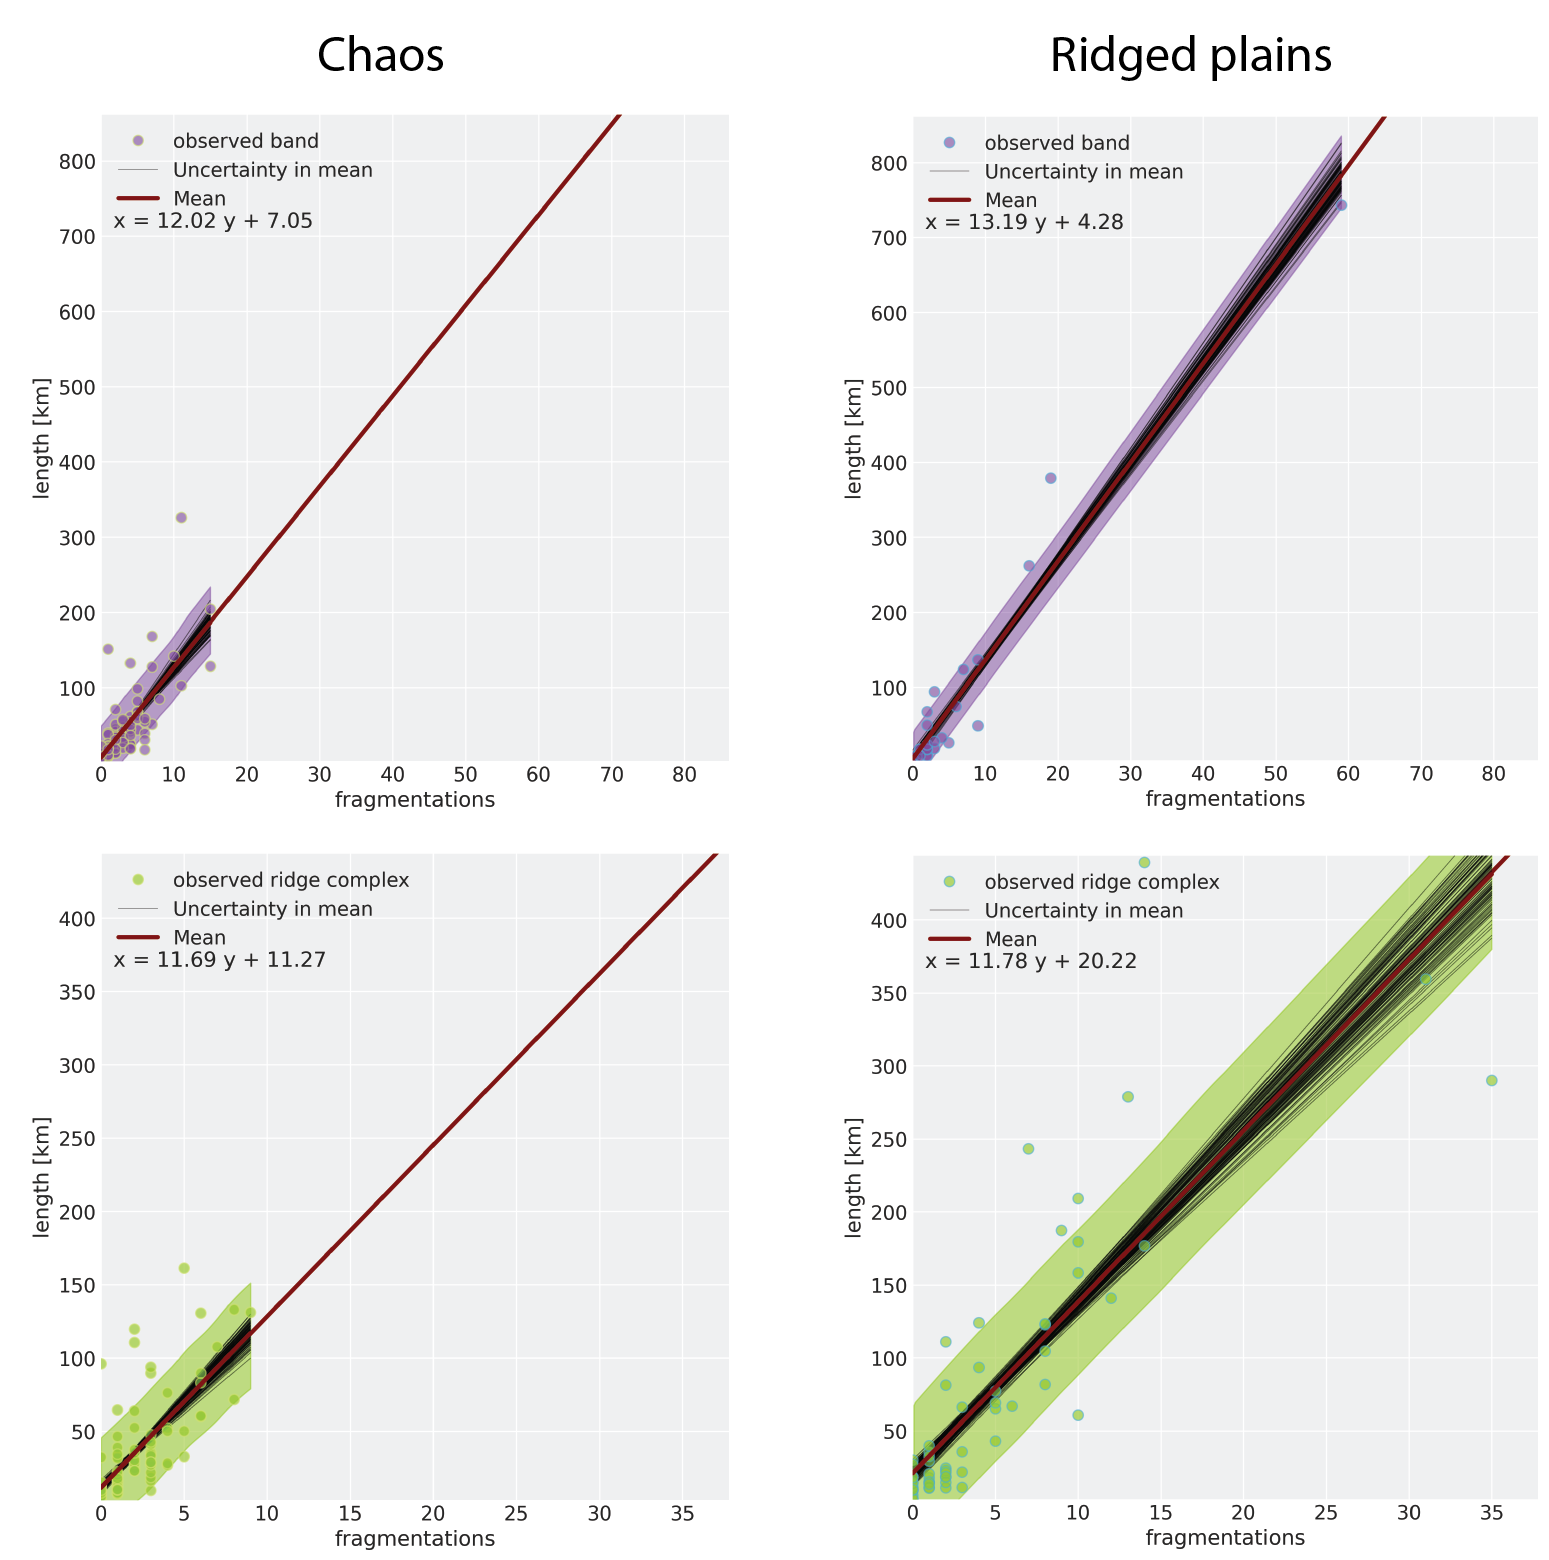
\includegraphics[width=\textwidth]{regional_mosaics/Figures/Bayes_analysis_regression_length_vs_fragm_band_rc.png}
%     \caption{Linear regression analysis for lineament length versus number of fragmentations, for \textbf{bands} and \textbf{ridge complexes}. The filled area shows the 97\% highest probability density interval of the posterior predictive samples (indicating where 97\% of the actual data are contained based on the posterior distribution).}
%     \label{fig_Bayes_length_frags_1}
% \end{figure*}
% \begin{figure*}
%     \centering
%     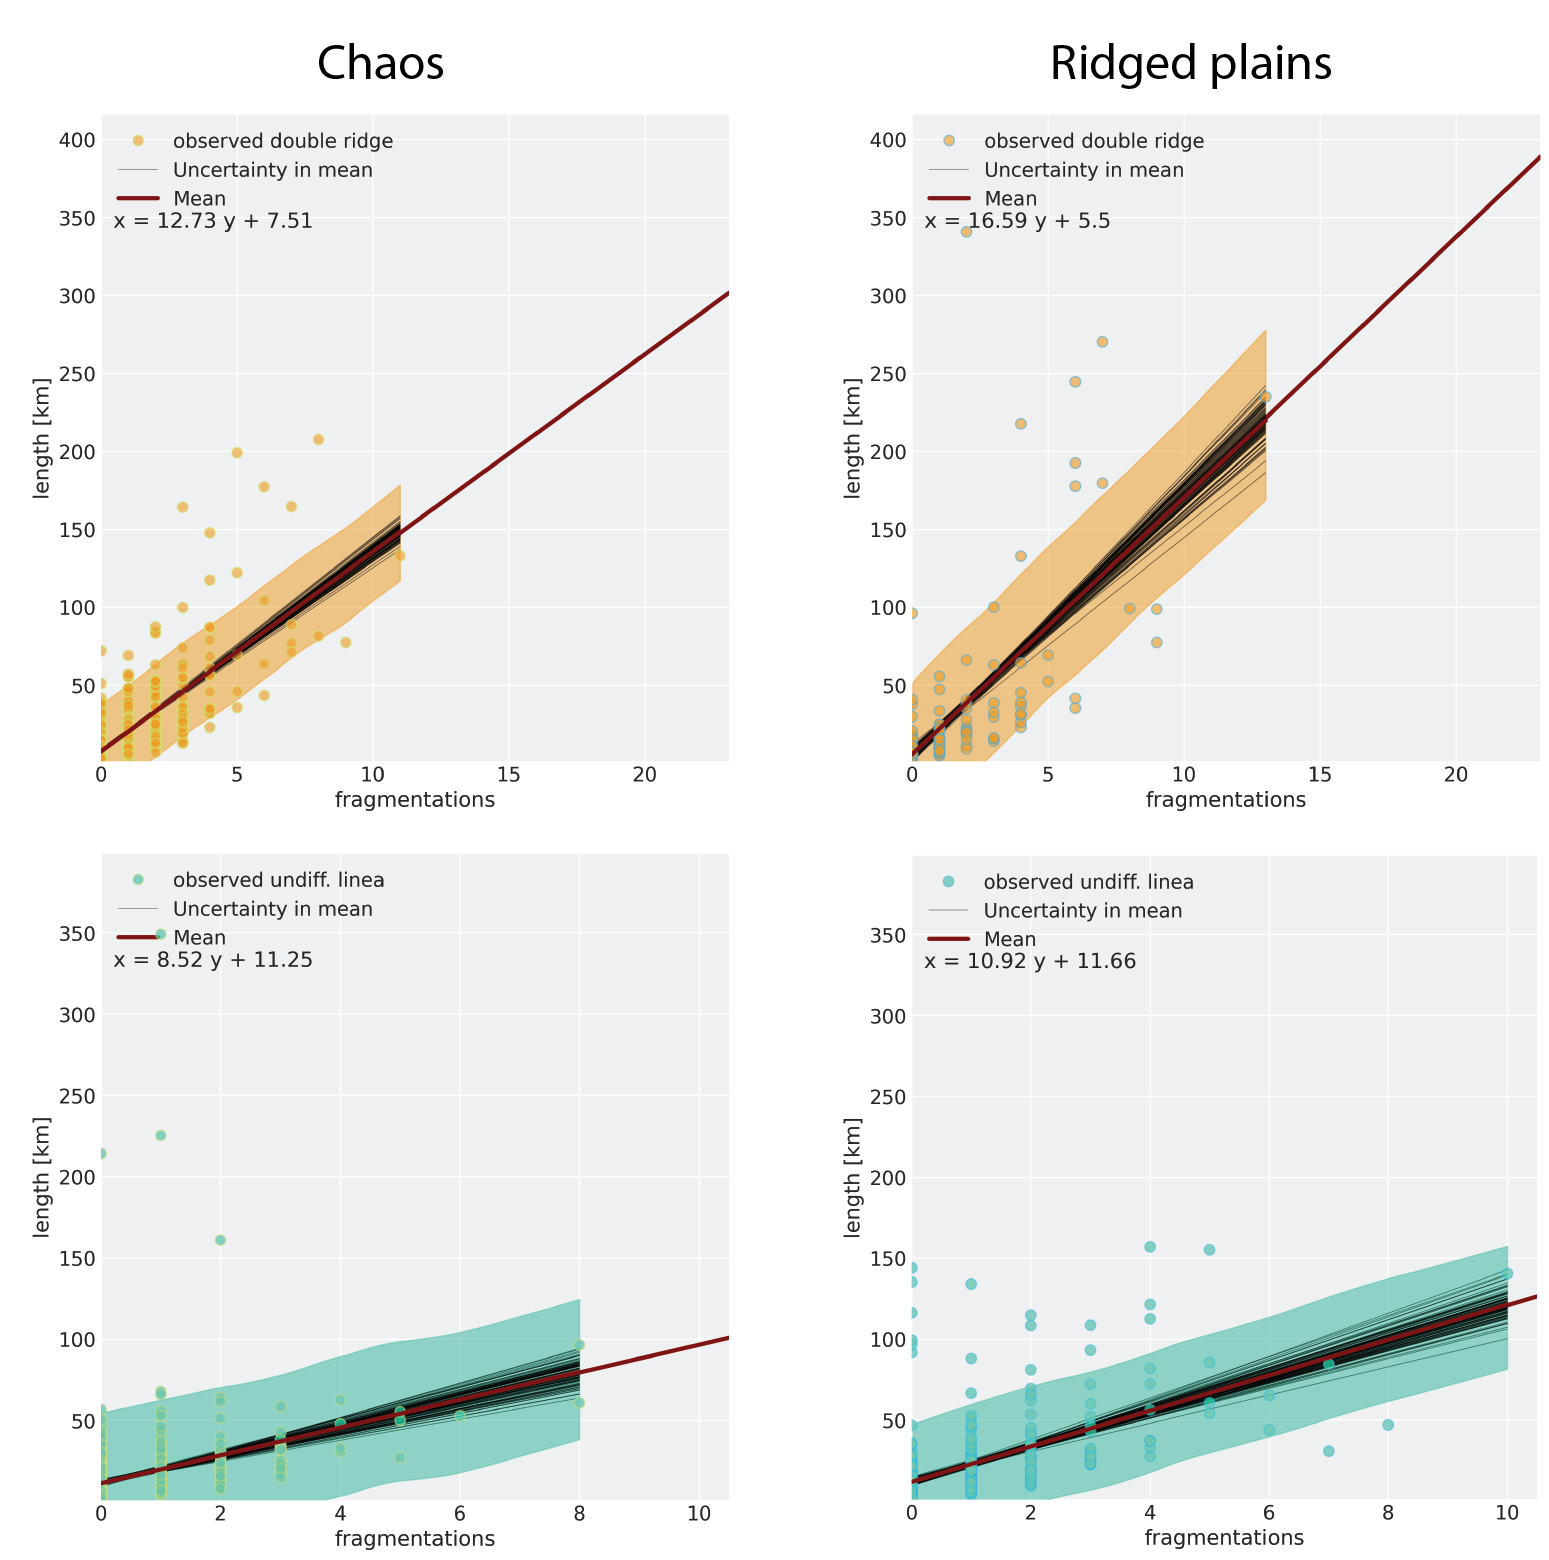
\includegraphics[width=\textwidth]{regional_mosaics/Figures/Bayes_analysis_regression_length_vs_fragm_db_ul.png}
%     \caption{Same as \Cref{fig_Bayes_length_frags_1} for \textbf{double ridges} and \textbf{undifferentiated lineae}.}
%     \label{fig_Bayes_length_frags_2}
% \end{figure*}
% 
% % legnth vs. FPK
% \begin{figure*}
%     \centering
%     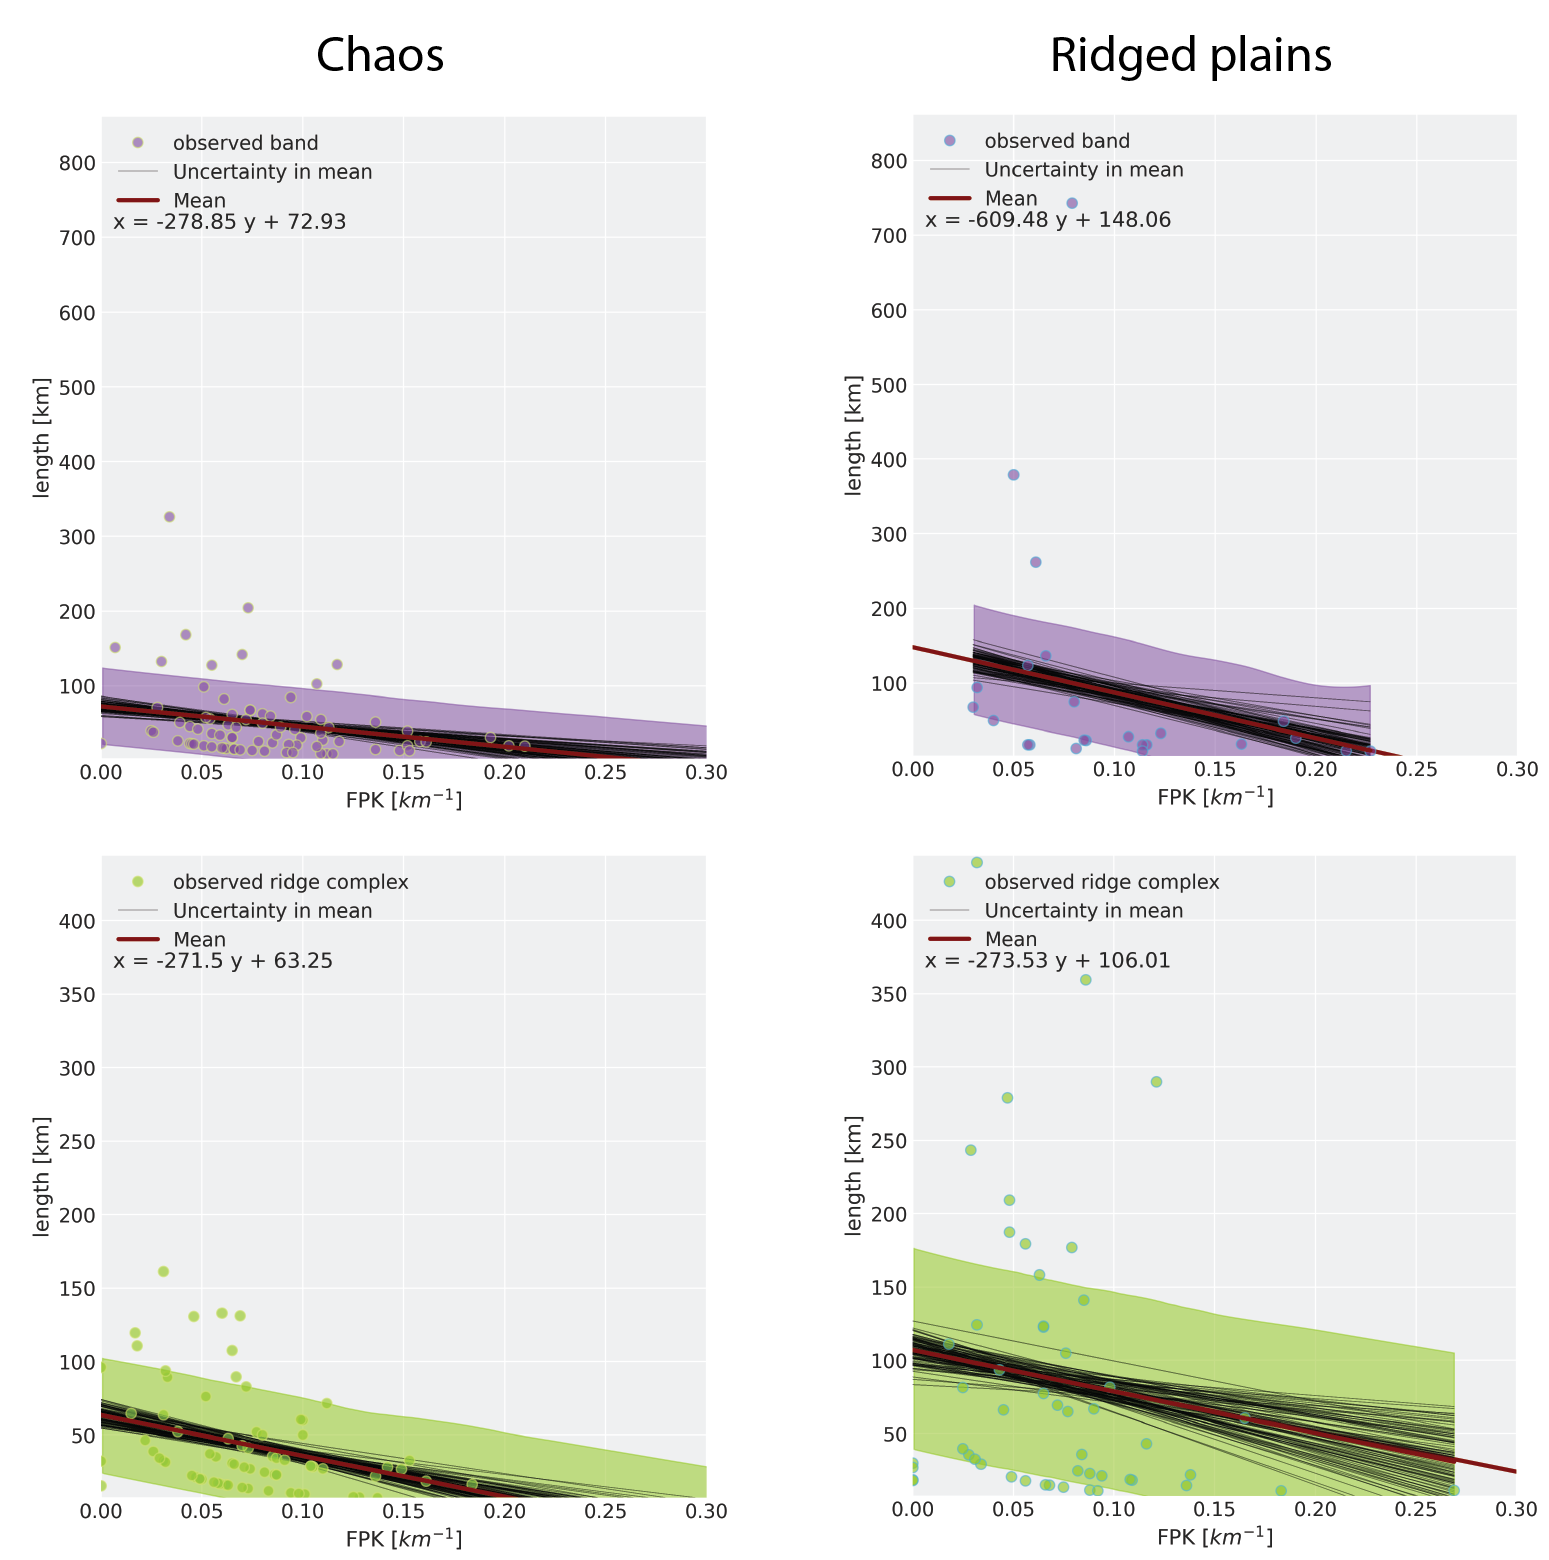
\includegraphics[width=\textwidth]{regional_mosaics/Figures/Bayes_analysis_regression_length_vs_FPK_b_rc.png}
%     \caption{Linear regression analysis for lineament length versus fragmentations per kilometre (FPK), for \textbf{bands} and \textbf{ridge complexes}. The filled area shows the 97\% highest probability density interval of the posterior predictive samples (indicating where 97\% of the actual data are contained based on the posterior distribution).}
%     \label{fig_Bayeslength_FPK_1}
% \end{figure*}
% \begin{figure*}
%     \centering
%     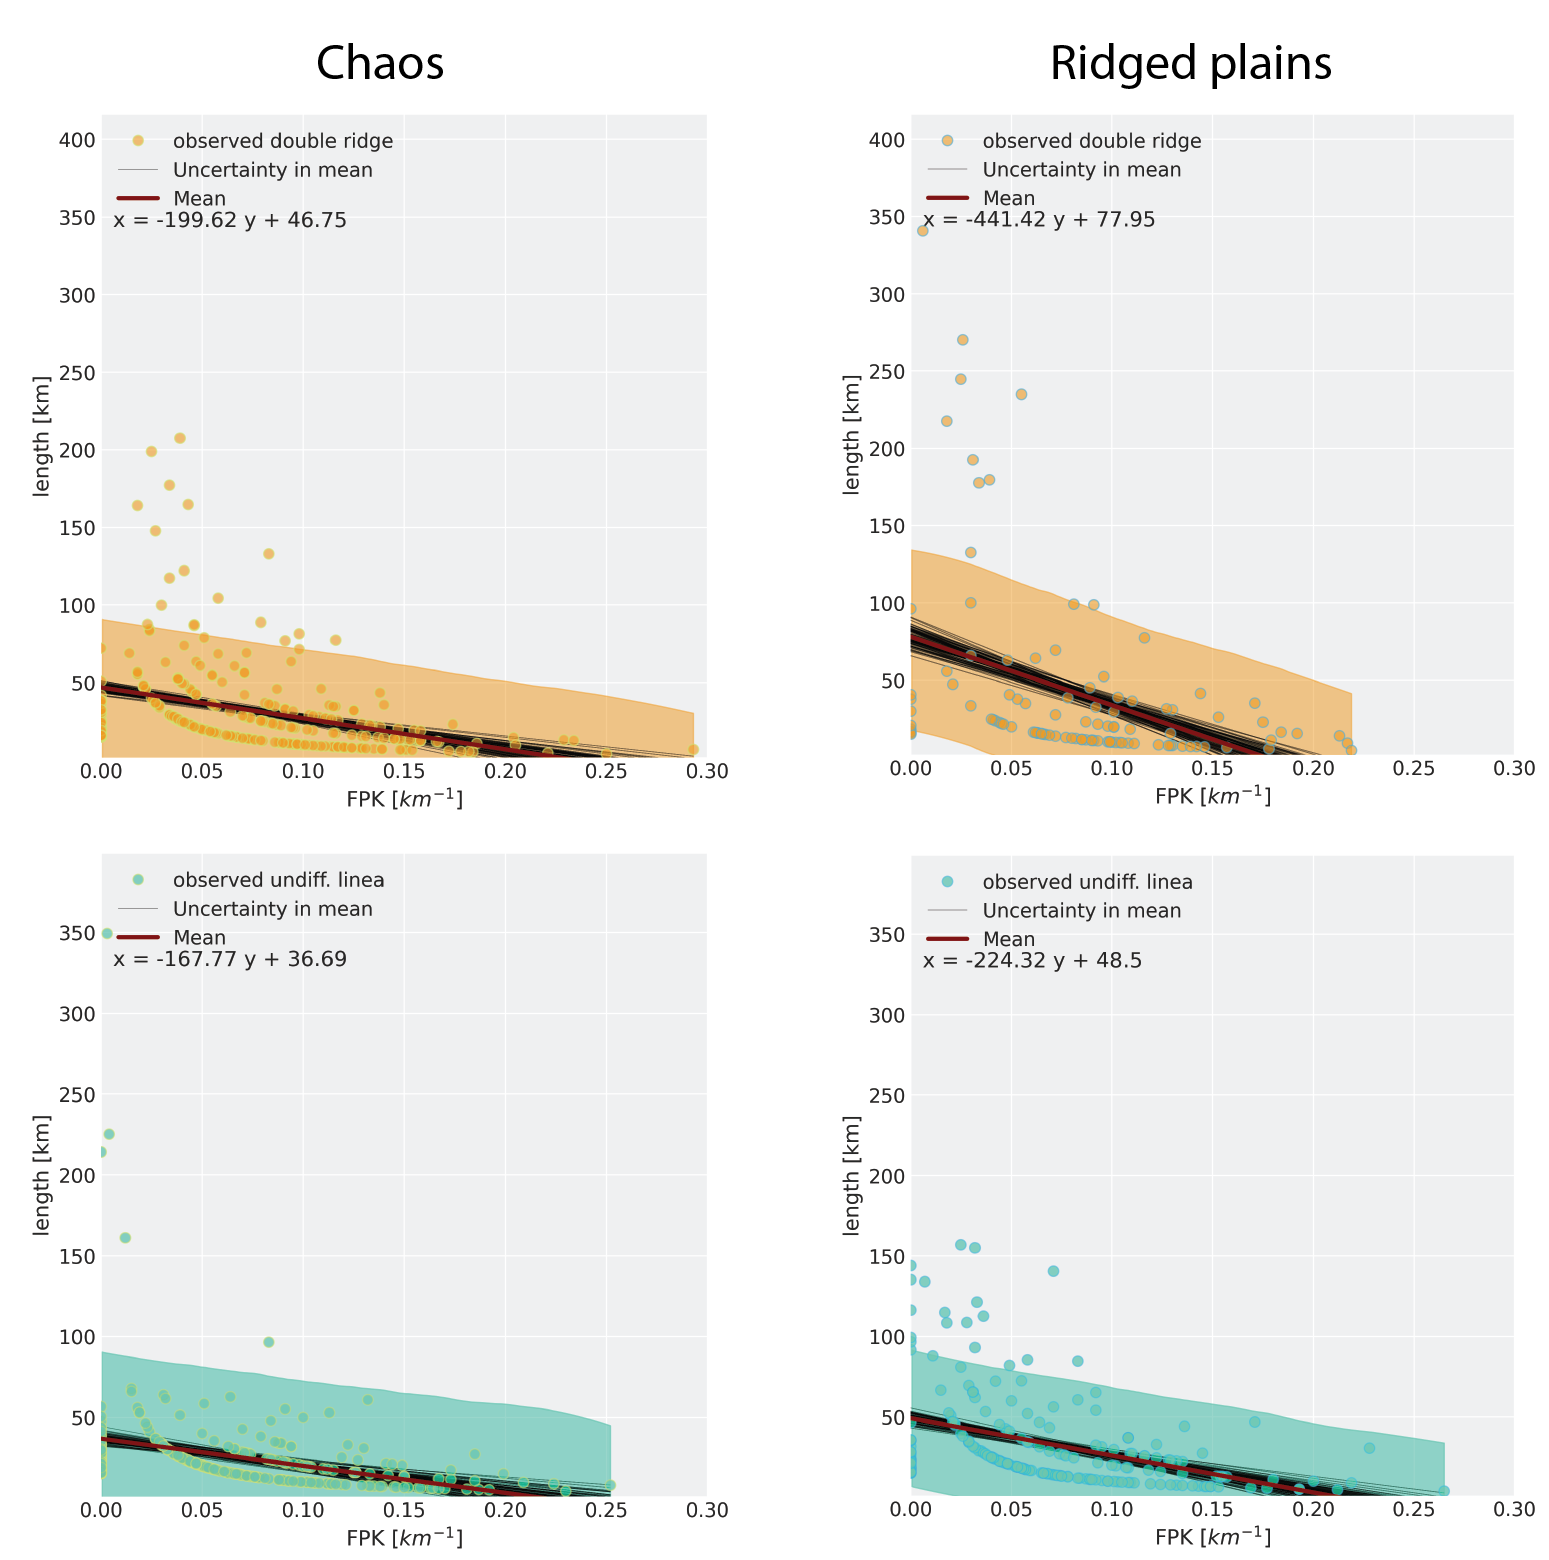
\includegraphics[width=\textwidth]{regional_mosaics/Figures/Bayes_analysis_regression_length_vs_FPK_db_ul.png}
%     \caption{Same as \Cref{fig_Bayeslength_FPK_1} for \textbf{double ridges} and \textbf{undifferentiated lineae}.}
%     \label{fig_Bayeslength_FPK_2}
% \end{figure*}
% 
% % width vs. FPK
% \begin{figure*}
%     \centering
%     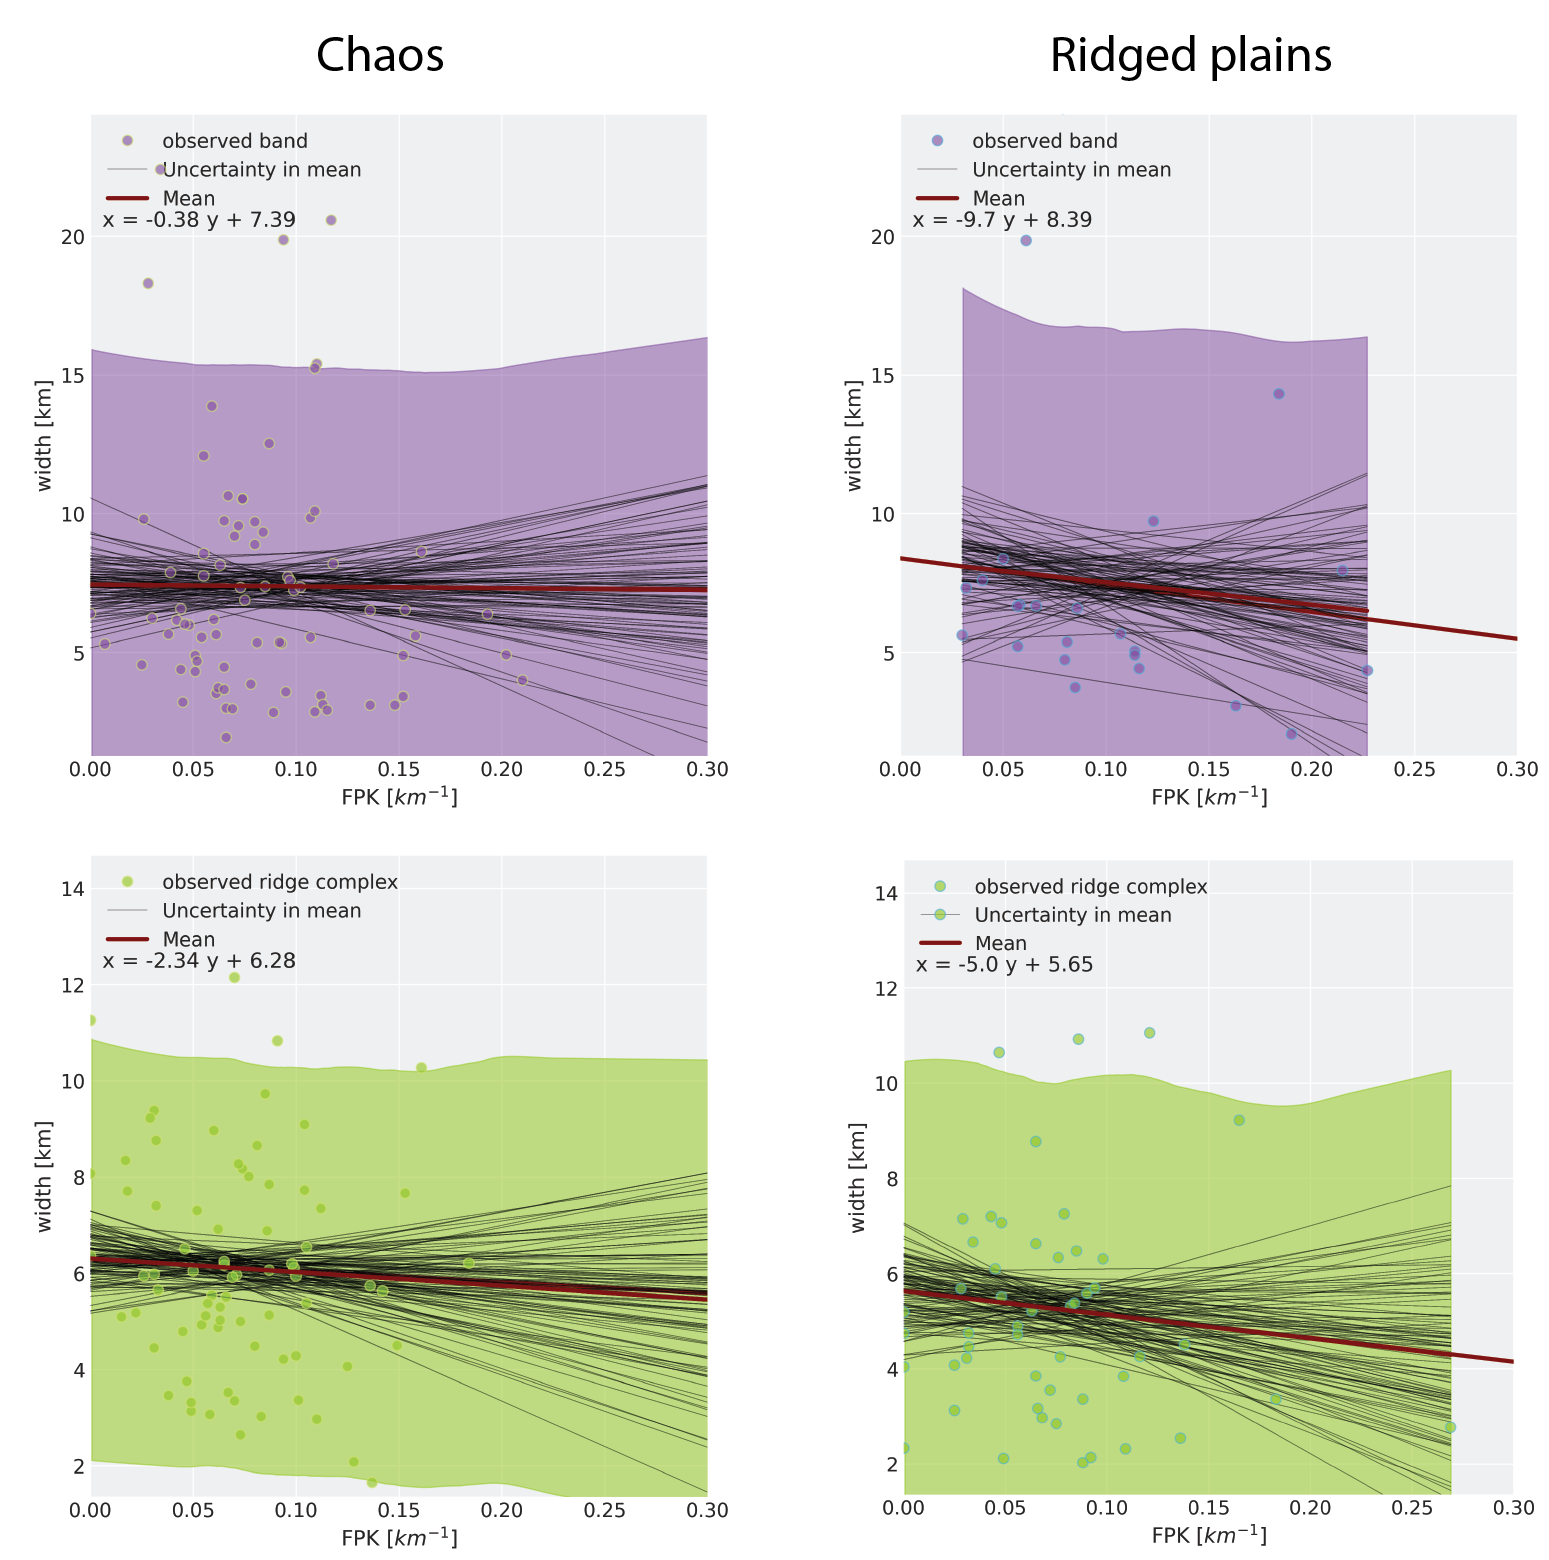
\includegraphics[width=\textwidth]{regional_mosaics/Figures/Bayes_analysis_regression_width_vs_FPK_b_rc.png}
%     \caption{Linear regression analysis for lineament width versus fragmentations per kilometre (FPK), for \textbf{bands} and \textbf{ridge complexes}. The filled area shows the 97\% highest probability density interval of the posterior predictive samples (indicating where 97\% of the actual data are contained based on the posterior distribution).}
%     \label{fig_Bayeswidth_FPK_1}
% \end{figure*}
% \begin{figure*}
%     \centering
%     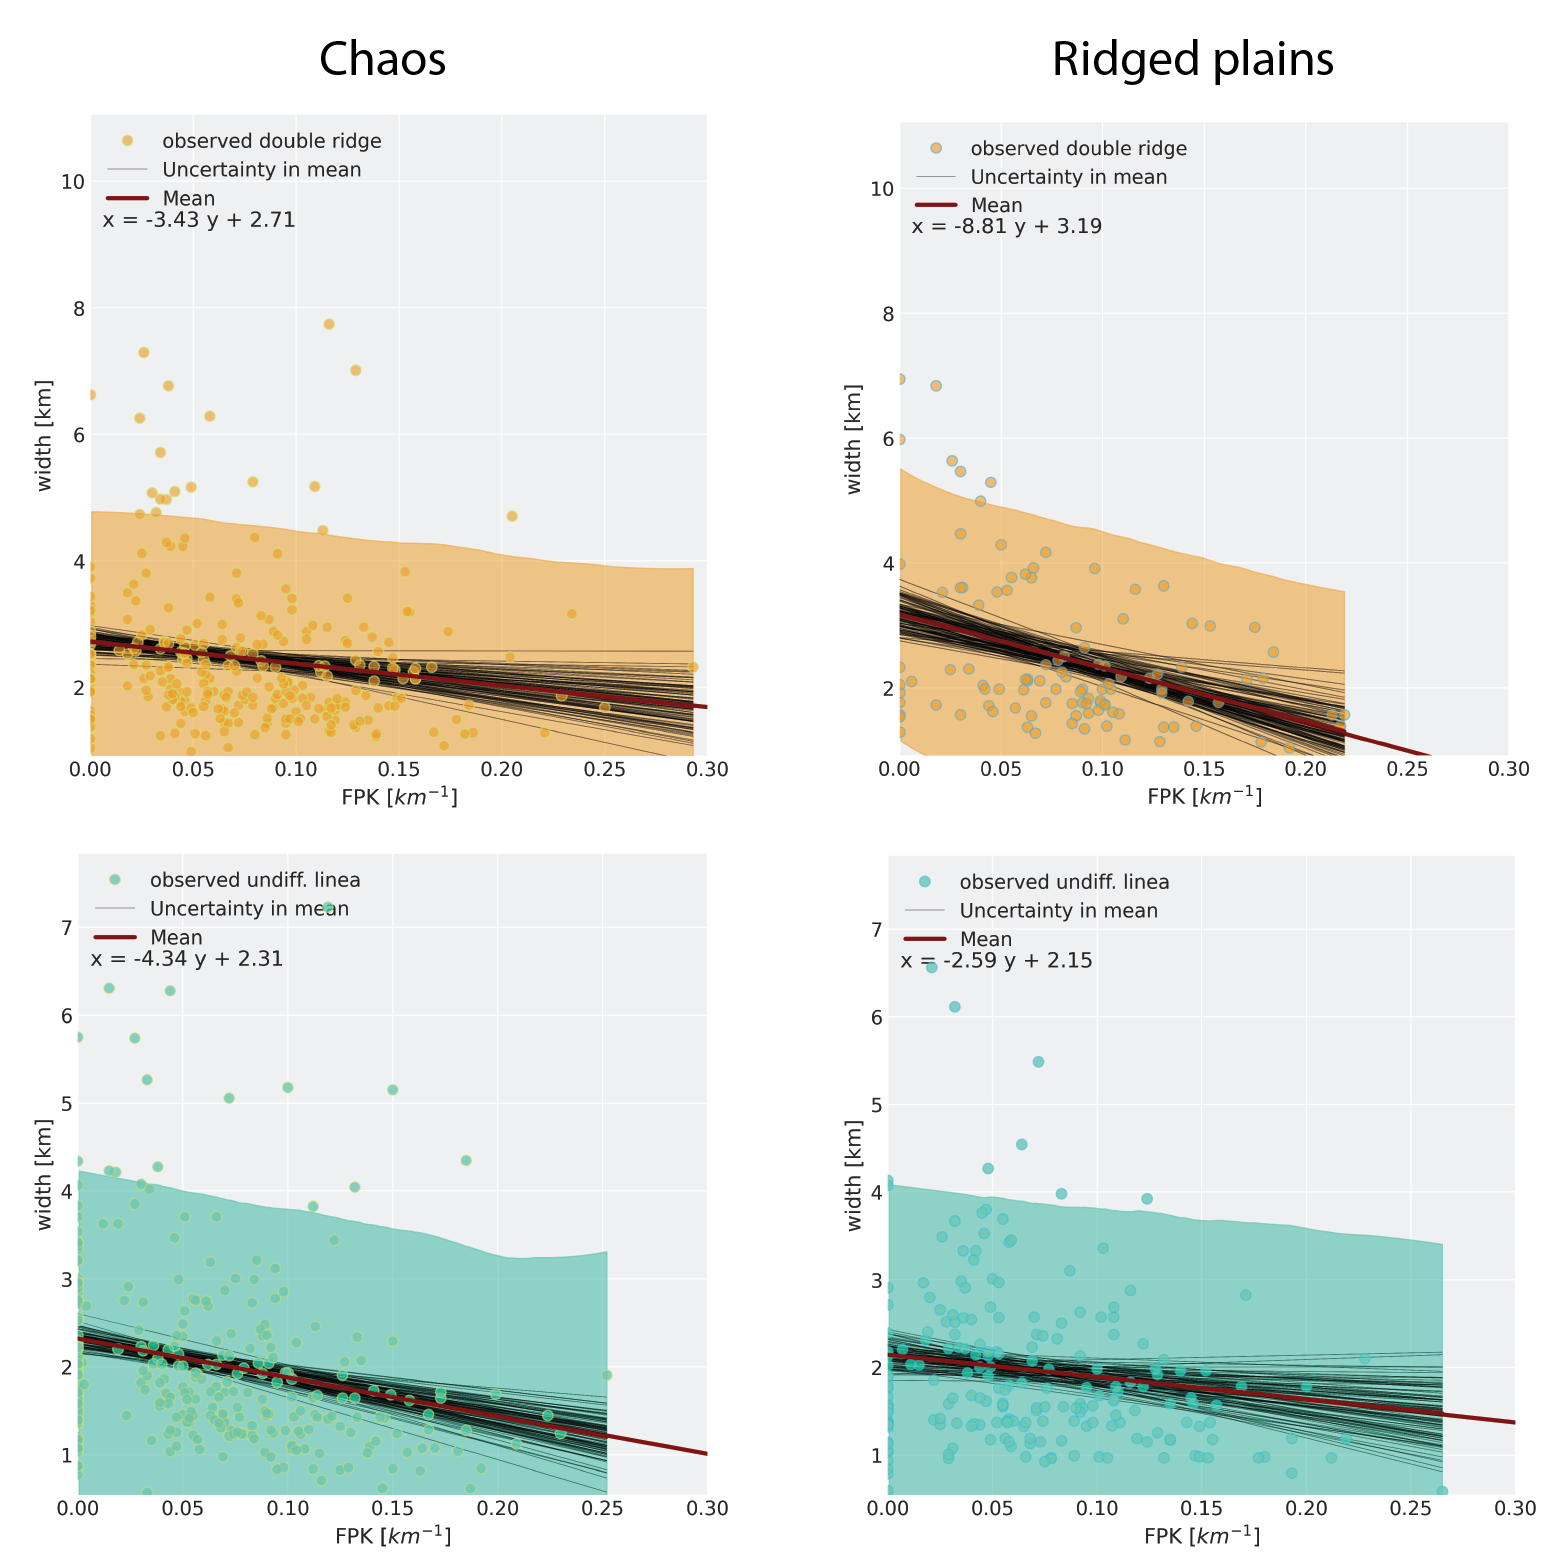
\includegraphics[width=\textwidth]{regional_mosaics/Figures/Bayes_analysis_regression_width_vs_FPK_db_ul.png}
%     \caption{Same as \Cref{fig_Bayeswidth_FPK_1} for \textbf{double ridges} and \textbf{undifferentiated lineae}.}
%     \label{fig_Bayeswidth_FPK_2}
% \end{figure*}
% 
% % width vs length
% \begin{figure*}
%     \centering
%     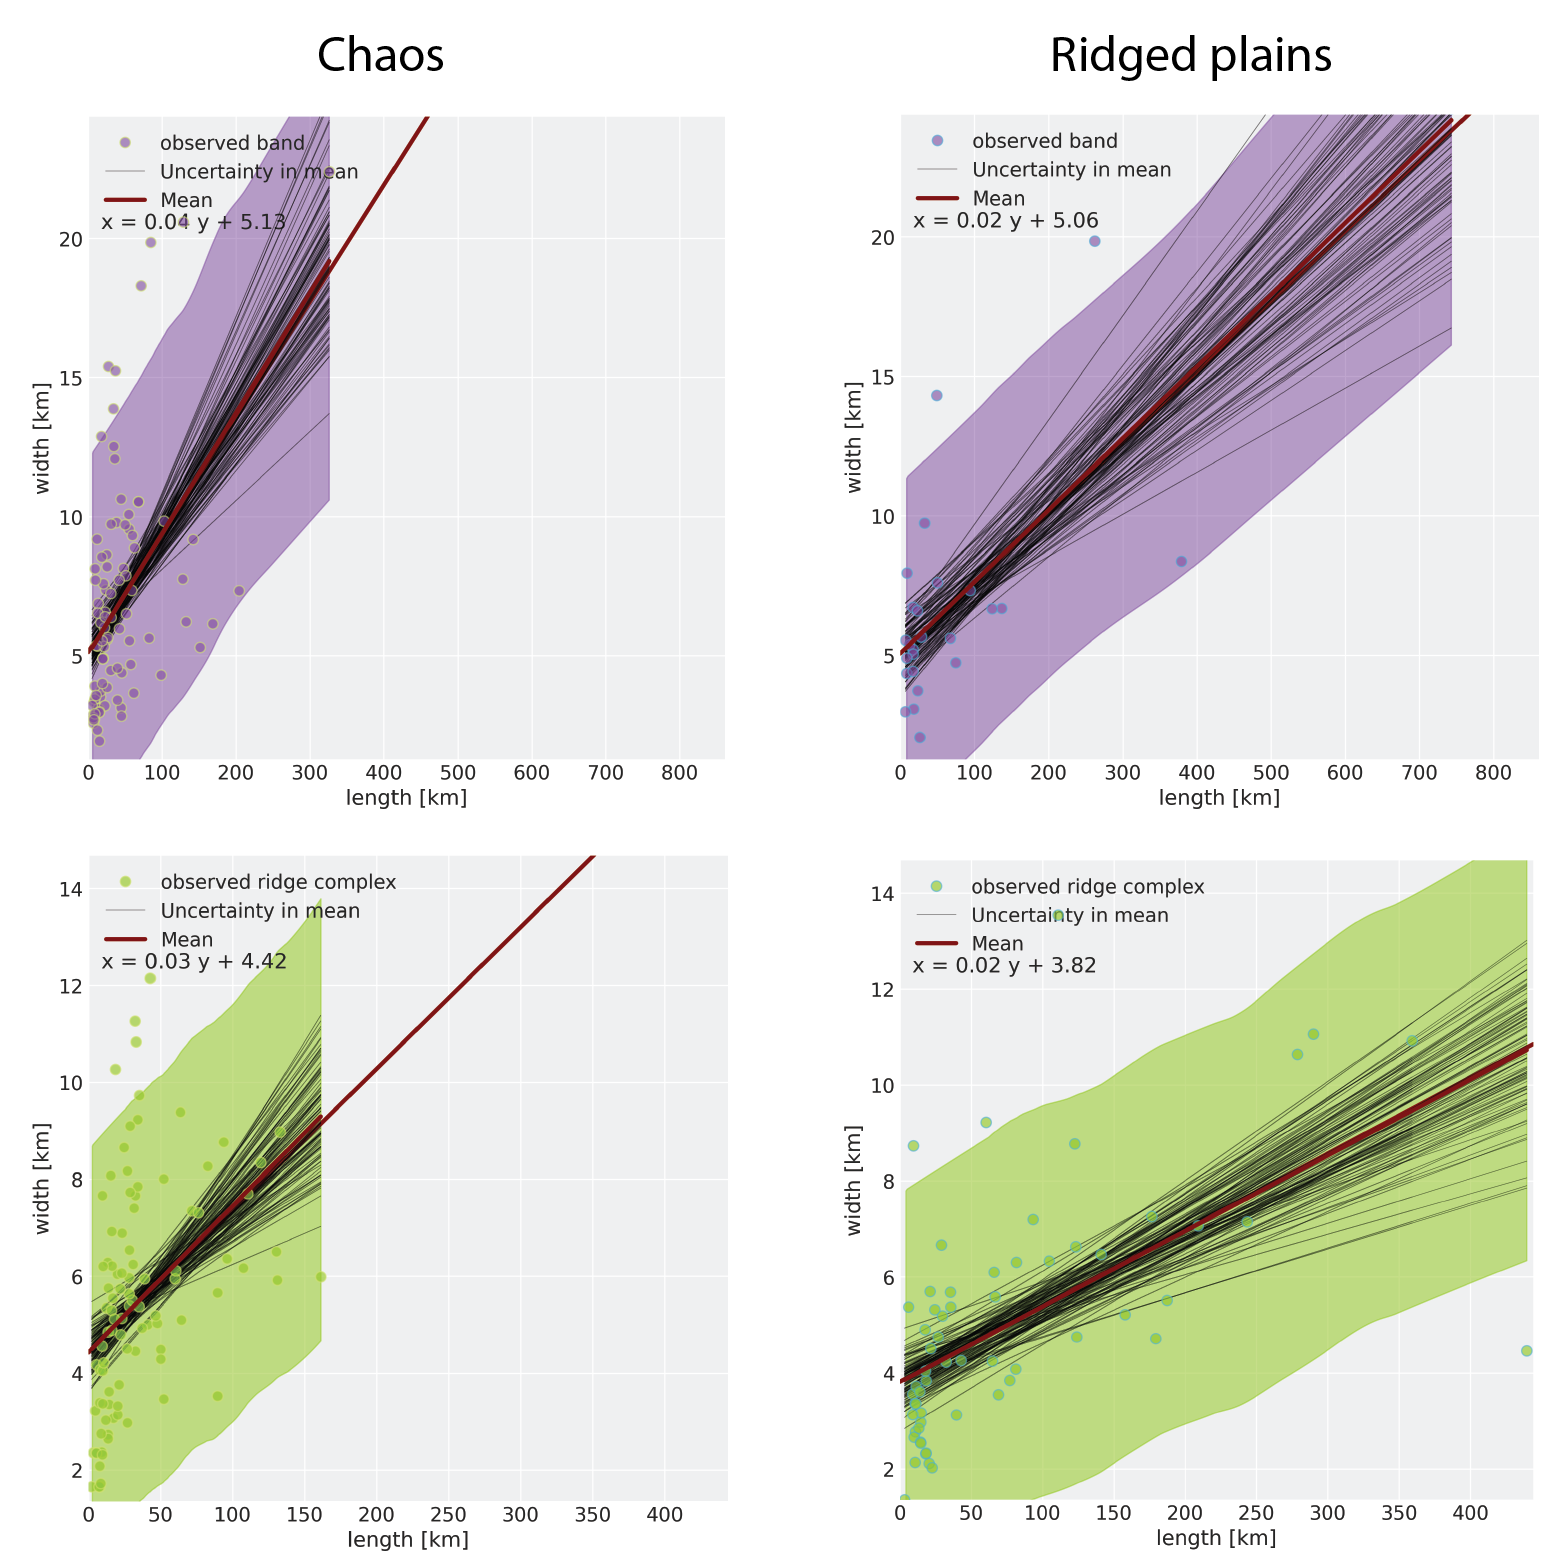
\includegraphics[width=\textwidth]{regional_mosaics/Figures/Bayes_analysis_regression_width_vs_length_b_rc.png}
%     \caption{Linear regression analysis for lineament width versus length, for \textbf{bands} and \textbf{ridge complexes}. The filled area shows the 97\% highest probability density interval of the posterior predictive samples (indicating where 97\% of the actual data are contained based on the posterior distribution).}
%     \label{fig_Bayeswidth_length_1}
% \end{figure*}
% \begin{figure*}
%     \centering
%     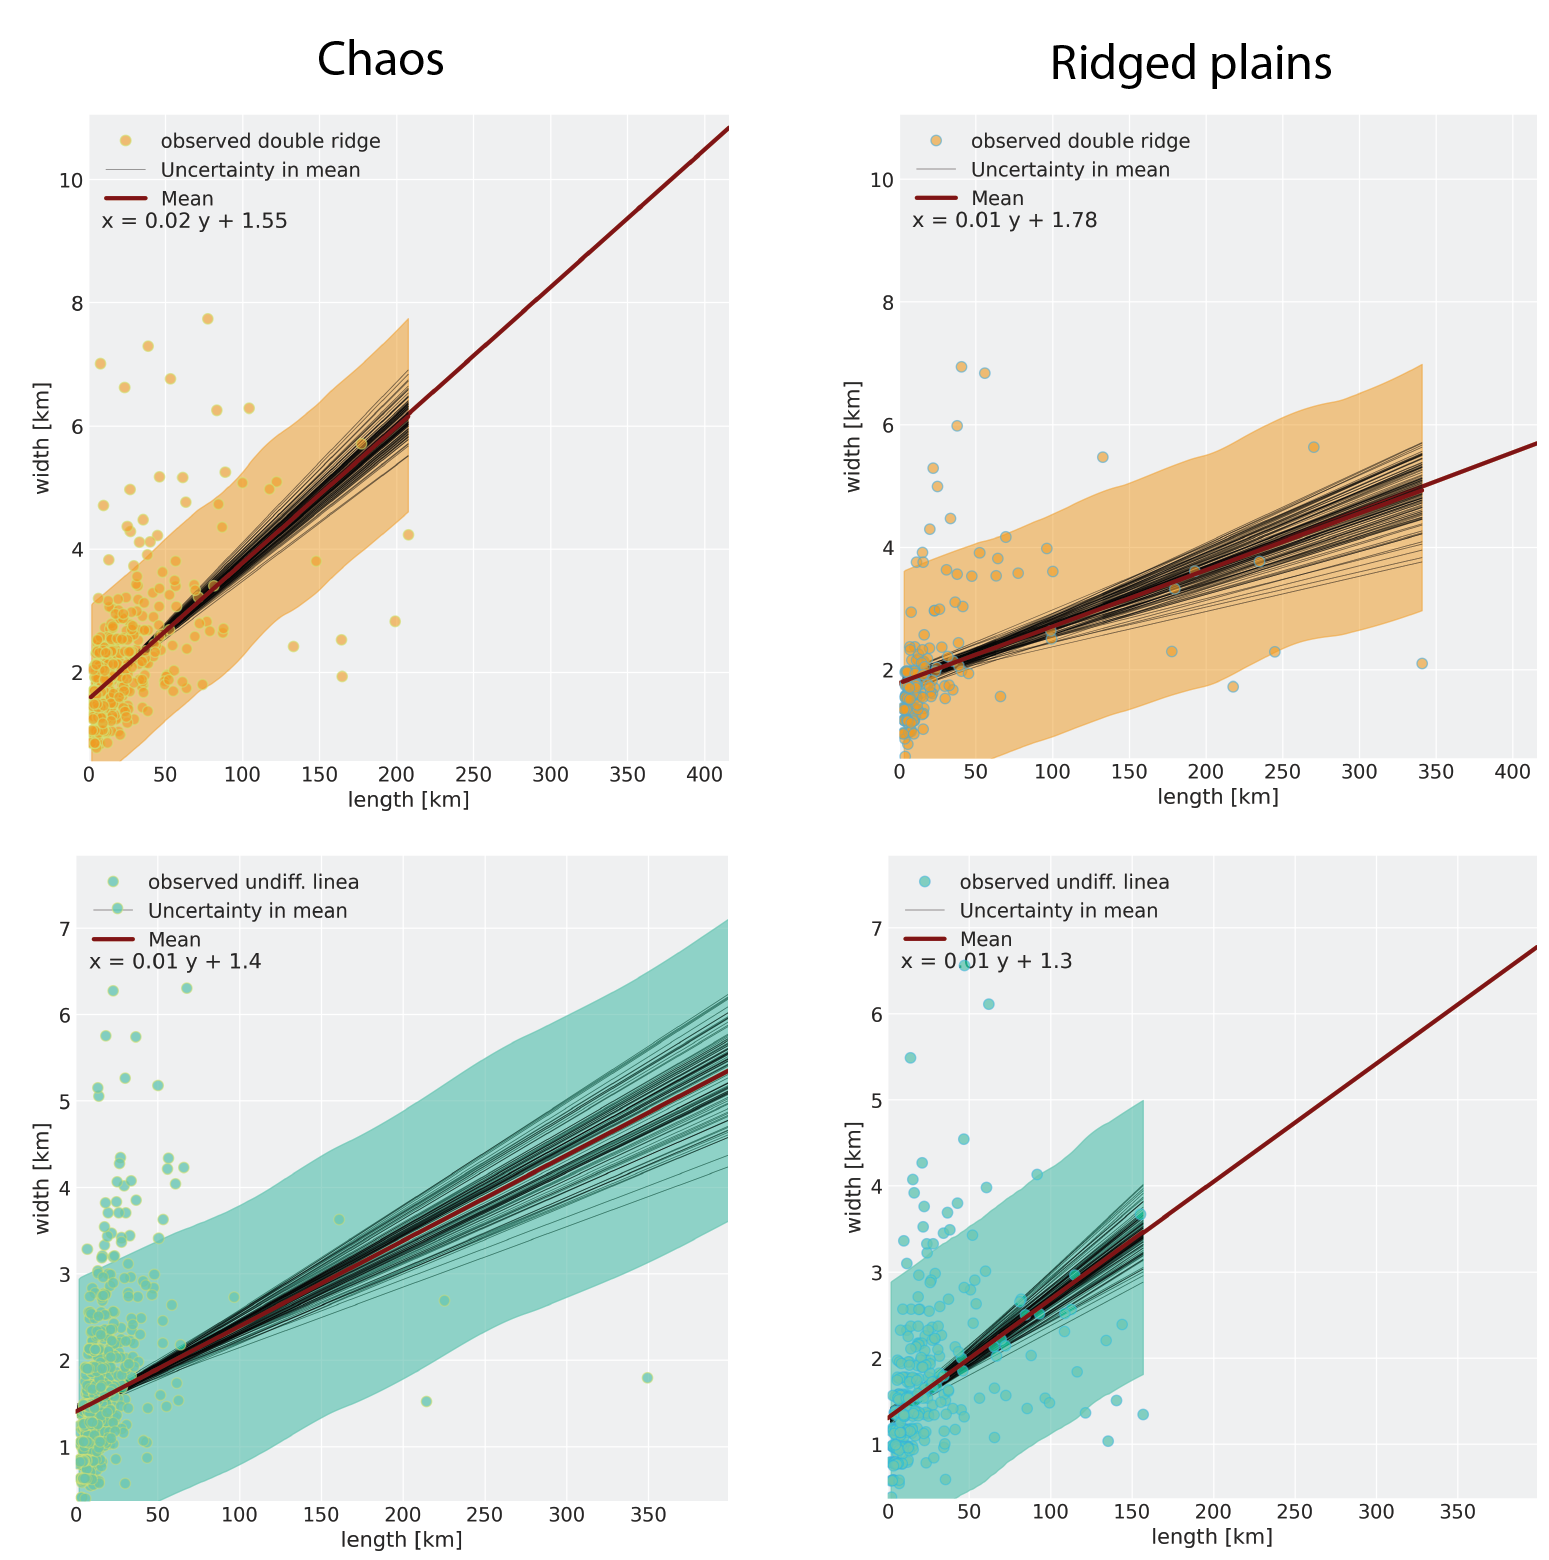
\includegraphics[width=\textwidth]{regional_mosaics/Figures/Bayes_analysis_regression_width_vs_length_db_ul.png}
%     \caption{Same as \Cref{fig_Bayeswidth_length_1} for \textbf{double ridges} and \textbf{undifferentiated lineae}.}
%     \label{fig_Bayeswidth_length_2}
% \end{figure*}


\paragraph{\textbf{Do we find correlations between lineament characteristics, and do the fits vary for the chaos and ridged plains unit?}} Short answer: We find a weak correlation between relative age and width (younger lineaments seem to be wider). Separated into categories, we find that wider linea are longer. Together, this shows that young lineaments are more likely to be long and wide, which could be an observation bias due to fading and fragmentation. The fits only slightly vary for chaos vs ridged plains.

In the following, we analyse how the extracted characteristics correlate with each other. We note that for correlations with FPK, we filtered out values with FPK$=$0 \textbf{and} length $<$30~km, because these lineaments might either be old and fragmented or young.

\paragraph{Length vs number of fragmentations:} 
The Bayesian linear regression fit of length versus number of fragmentations (Figs.~12 and~13 in the original publication) shows that for most lineaments, a linear correlation of length and number of fragmentations provides a good fit. The slopes are flattest for undifferentiated lineae. Chaos and ridged plains show significant differences in slopes for double ridges and undifferentiated lineae when compared category-wise\sidenote{As shown in Table~17 in the supplementary material of the original publication.}. The ranges of slopes for different categories (9.6 to \qty{14.7}{\km}) are higher than between chaos and ridged plains (max. \qty{4}{\km} difference in slope, for double ridges).

\paragraph{Length vs FPK:} 
We would expect to see no correlation for length vs. FPK (Figs.~14 and~15 in the original publication), if the number of fragmentations is positively correlated to the number of fragmentations. However, we observe a residual, negative correlation of length with FPK, simply because not all lineaments lie on one line. More values with a low FPK lie outside the 97\% highest probability density interval (HDPI), which should capture 97\% of the distributed data. Since the number of fragmentations is discrete, we see constant, exponentially decreasing lines. The negative correlation means that longer linea are disproportionally young, which is either an observation bias, potentially due to fading\sidecite{Bierhaus2009}, or a bias from connecting lineaments, if heavily fragmented lineae are too fragmented to show their continuation. Overall, chaos shows slopes closer to zero than ridged plains. The closest to a slope of zero get undifferentiated lineae in chaos terrain. The maximal negative slope is exhibited by bands in ridged plains.

\paragraph{Width vs FPK:} 
Correlating width with FPK (Figs.~16 and~17 in the original publication) tries to answer the question: Are older lineaments wider or narrower? In general, older lineaments seem to be narrower, but the uncertainty is large and there might be no underlying real-world correlation. The most constrained negative correlation is exhibited by double ridges in ridged plains. Slopes for bands and ridge complexes range from negative to positive within their 97\% HDPI, for both chaos and ridged plains. The slopes of double ridges and undifferentiated are negative within their 97\% HDPI. The negative correlation, after an observational bias indicated by length vs FPK is excluded, could either indicate that more recently formed double ridges and undifferentiated lineae develop into wider lineaments, or that throughout the evolution of double ridges and undifferentiated lineae, the width decreases, hinting at the possibility of subduction or shrinking (also in the vertical) due to a weakening of driving forces, such as changing shear forces\sidecite{Gaidos2000, Nimmo2002, Han2008}.

\paragraph{Width vs length:} A possible correlation of width with length can answer the question: Are longer lineaments also wider? Or are longer lineaments narrower?  We find that, separated into categories, longer linea are wider (Figs.~18 and~19 in the original publication). However, the scatter plots show a wide range of widths for short lineaments, which is not fully captured by the linear regression line, but only in the HDPI. If longer lineaments ($>$\qty{50}{\km}) would be excluded, correlations would be weaker. This means that short lineaments can have any width, while long lineaments are not especially narrow. Nevertheless, slopes are higher (longer lineaments are even wider) in chaos terrain, although the comparison is flawed by the fact that lineaments in chaos terrain are generally shorter. The effect of longer and wider lineaments is most pronounced for bands in chaos terrain. We speculate that if the ice fails in a way that allows a long crack to result (e.g. if a higher pressure builds up for a long crack to form), the crack might also penetrate deeper than shorter cracks, which could result in wider lineaments, because the crack stays active for longer. However, this preliminary result needs to be validated, for example with lineament age sequences to better quantify the relation of age and length.\\

The scatter plots in Figs.~16 and~17 in the original publication show in more detail than \Cref{fig:grid_chaosvspr}.c that the FPK reaches higher values in chaos terrain.

\subsubsection{Discussion of the revised lineament map}\label{sec:discussing_revisedMap}
The question that arose most often during revision of the southern leading hemisphere RegMap 17ESREGMAP02 was about the differentiation of bands and ridge complexes. For one, morphologies of ridged bands and ridge complexes are similar, while other types of bands, e.g. smooth bands\sidecite{ProckterPatterson2009}, are distinct. Adding band sub-categories to LineaMapper might help to increase performance, although increasing number of categories does not always lead to better classification. Since some bands appear bright in infrared wavelengths\sidecite{DoggettEuropaBook2009}, LineaMapper could be trained to take in spectral information, for example from Galileo Near Infrared Mapping Spectrometer (NIMS) observations. During the Europa Clipper mission, EIS can be combined with spectral data from the Mapping Imaging Spectrometer for Europa\sidecite{Blaney2022} datasets could be combined and input together into LineaMapper.

Furthermore, a finer distinction of band types would lead to further statistical insights. With the current categorisation, we observe similar distributions for bands-ridge complexes and double ridges-undifferentiated lineae. This could imply that most undifferentiated lineae would resolve as double ridges or share the same formation mechanism, while for bands and ridge complexes, they are either hard to distinguish by their morphologies or form similarly\sidecite{Patterson2010}. 

However, there is one interesting difference to ridge complexes. The fact that bands are widest and have the highest FPK values, which means they are on average oldest, might indicate that bands formed earlier and became wider than any other category. % This result is in line with .

We characterize the nature of fragmentation processes in ridged plains and chaos terrain.
We find higher chaos vs. ridged plains differences for bands and ridge complexes than for undifferentiated lineae and double ridges. Most striking is the almost identical width distribution of undifferentiated lineae and double ridges.
Together with the observation of an absence of young bands in ridged plains, we hypothesise that more recently formed features survive disruption during chaos formation better, maybe simply because they have locally the highest elevation, or the composition and porosity withstands chaos disruption more likely. However, it could also be that older lineaments blend in easier with the chaos matrix, which leads to an observational bias.  

The slopes of length fit by number of fragmentations could be taken to work out a refined, category-wise FPK, which could capture the differences in how lineaments are fragmented. The exponentially decreasing slopes of length vs FPK could tell us that the FPK should rather be calculated by the length divided by the logarithm of the number of fragmentations. On the other hand, this might be an observational bias, likely due to resolution, which prevents a full record of fragmentations. A higher resolution dataset will shed light on this matter. The possible negative correlation of width vs FPK (younger lineaments are wider) needs verification with an established age sequence. The positive correlation of width with length (longer linea are wider) could be confirmed on other parts of the RegMaps, and possible explanations should be investigated.
We note that, as a preliminary result, we do not find any significant correlation of radiance with FPK for any category when we evaluate the photometrically corrected images (not shown).

We empirically find that fine cracks (troughs) can be identified by filtering for undifferentiated lineae with a length greater than 150~km. Out of these long cracks, the youngest ones can be identified by width $\leq$ 3~km and FPK $<$ 0.03 fragmentations per kilometer. With this, LineaMapper will be useful for recent trough identification in EIS images.

\plainwidefig{1}{regional_mosaics/Figures/LM1_1_polygon_foroverleaf.png}{Fully-automatically produced lineament map of the Galileo RegMaps with \textbf{LineaMapper v1.1}. A) RegMap of the anti-jovian, trailing hemisphere. B) RegMap of the leading hemisphere. The absence or reduced density of lineaments concurs with the presence of chaos terrain. C) Excerpt of the leading hemisphere. A unit of chaos terrain is left blank, i.e. LineaMapper does not confuse chaos terrain with lineaments here. D) Excerpt of the trailing hemisphere with all four categories predicted by LineaMapper.}{fig:raw_regmaps_LM1.1}


\plainwidefig{1}{regional_mosaics/Figures/LM2_0_polygon_foroverleaf.png}{Fully-automatically produced lineament map of the Galileo RegMaps with \textbf{LineaMapper v2.0}. A) RegMap of the anti-jovian, trailing hemisphere. B) RegMap of the leading hemisphere. The absence or reduced density of lineaments concurs with the presence of chaos terrain. C) Excerpt of the leading hemisphere. A unit of chaos terrain is left blank, i.e. LineaMapper does not confuse chaos terrain with lineaments. D) Excerpt of the trailing hemisphere with all four categories predicted by LineaMapper.}{fig:raw_regmaps_LM2.0}

\plainwidefig[t]{1}{regional_mosaics/Figures/trailing_geounits.png}{Predicted geological units (chaos, transition unit, ridged plains) on the trailing RegMap by the lineament density extracted from LineaMapper v1.1 and v2.0 predictions. For comparison, the global geologic map~\cite{Leonard2024} is shown on the right with the outline of the analyzed SSI images.}{fig_trailing_chaos_pr_predicted}

\subsubsection{Fully automatic RegMaps lineament map}\label{sec:fullRegMaps}

Based on tests with photometrically corrected input data, we decide to use the 149 non-corrected ``native'' Galileo SSI images that constitute the RegMaps for inference with LineaMapper v1.1 and v2.0. The stitched LineaMapper output on the RegMaps is shown in \Cref{fig:raw_regmaps_LM1.1} for v1.1 and in \Cref{fig:raw_regmaps_LM2.0} for v2.0. The two predictions are qualitatively similar. This also manifests in the resulting number of predictions: we retrieve 133,801 stitched predictions with LineaMapper v1.1 and 134,101 predictions with LineaMapper v2.0. As an example, LineaMapper v1.1 needed 6 minutes for prediction and stitching of Galileo image with SSI ID \texttt{C0449961814R} on one CPU. 

\plainwidefig[t]{1}{regional_mosaics/Figures/leading_geounits.png}{Predicted geological units (chaos, transition unit, ridged plains) on the leading RegMap by the lineament density extracted from LineaMapper v1.1 (LM1.1, on the left) and v2.0 (LM2.0, middle) predictions. For comparison, the global geologic map\cite{Leonard2024} is shown on the right with the outline of the analysed SSI images.}{fig_leading_chaos_pr_predicted}

\paragraph{\textbf{Can LineaMapper identify different terrain types (chaos and ridged plains) by lineament density?}}\label{sec:Q1LM_terraintypes}
Short answer: Yes, LineaMapper can be used to distinguish chaos and ridged plains based on the total lineament density, inferred by transforming LineaMapper into a pixel segmentation tool.


Because LineaMapper respects chaos terrain also in regions it has not seen before\sidenote{C side of \Cref{fig:raw_regmaps_LM1.1,fig:raw_regmaps_LM2.0}}, we qualitatively observe different densities within the RegMaps\sidenote{Portion AB of \Cref{fig:raw_regmaps_LM1.1,fig:raw_regmaps_LM2.0}}. In the following, we explore in more detail how the lineament density relates to chaos and ridged plains units mapped in the global geologic map\sidecite{Leonard2024}. 

We use the manually validated lineament density fingerprint of chaos and ridged plains terrain established in the previous section, which leads to the conditional classification eluded in \Cref{tab:condition_ch_pr}. For each analysed Galileo SSI image, we extract one lineament density value. This extracted lineament density value leads to the classification of the Galileo SSI image. Density values of $\leq$35.0\% are classified as chaos terrain, while densities $\geq$45.0\% are classified as ridged plains. Densities in between are labelled ``transition terrain'', which captures uncertainty in classification. The results are shown for the leading Regmap in \Cref{fig_leading_chaos_pr_predicted}, and for the trailing RegMap in \Cref{fig_trailing_chaos_pr_predicted}. Qualitatively, we see good agreements between the two LineaMapper versions as well as good agreement between LineaMapper predictions and the global geologic map by\sidecite{Leonard2024}. LineaMapper v2.0 predicts more transition terrain than v1.1. Given the almost equal amount of predictions, we conclude that the area of individual predictions is smaller (less complete) for v2.0 compared with v1.1. This is in line with results from \Cref{sec:lineamapper_compar}. Therefore, LineaMapper v1.1 results in slightly better predictions, especially on the trailing RegMap (\Cref{fig_leading_chaos_pr_predicted}). We find that if chaos units mapped in\sidecite{Leonard2024} are smaller than one frame, the prediction for this frame is either chaos terrain or transition terrain. There are few cases where no chaos terrain is mapped in a frame predicted as chaos terrain. Disagreement is found for the southern leading hemisphere, where mottled chaos material extends from the equatorial region in a lobate shape. It can be seen also in the revised lineament map (\Cref{fig:full_map}) that the lineament density is higher in this lobate extension than in the northward mottled chaos region. 

\begin{margintable}[]\scriptsize
\caption{Condition for distinguishing terrain types fully-automatically with LineaMapper.}
\label{tab:condition_ch_pr}
\begin{tabular}{@{}ccc@{}}
\toprule
lineament \\ density & predicted terrain \\ \midrule
0.0 - 35.0\% & Chaos \\
35.0 - 45.0 \% & transition terrain \\
45.0 - 100 \% & ridged plains \\ \bottomrule
\end{tabular}
\end{margintable}

\subsubsection{Discussion of the fully automatic RegMaps lineament map}
Comparison of LineaMapper's automatically generated mosaics (\Cref{fig:raw_regmaps_LM1.1,fig:raw_regmaps_LM2.0}) with previous maps of the RegMaps\sidecite{Figueredo2004} shows a higher level of detail traded with a less detailed distinction of different categories. Luckily, re-labelling is less time-intense than mapping new lineaments. Furthermore, other features, such as pits and domes, can be added to the fully-automatically retrieved lineament maps. 

Also in the full RegMaps output, we find the same qualitative differences between LineaMapper v1.1 and v2.0: output by v2.0, which is based on the transformer model SAM, is less continuous and provides less mask coverage, than output by v1.1. We conclude that v1.1, which is based on the Mask R-CNN, is up to now the better lineament mapping assistant out of the two versions. This could change with improved usage of SAM for LineaMapper. Nevertheless, having two fundamentally different models helps verification of the output, especially if manually labelled boxes are fed into LineaMapper v2.0, instead of the boxes output by v1.1.

Since the output of LineaMapper v1.1 and v2.0 is patchy, we are using their output as a pixel segmentation tool. An improved stitching algorithm, perhaps with specific conditions for each category or iterative stitching, could resolve this issue, which enables a more robust estimation of length, width, and number of fragmentations to search for example for latitudinal variations or leading/trailing differences, which would open the floor for latitude-dependent cracking or evolution mechanisms. However, we stress that any result would need to be manually revised or verified from a different source. 

The output of LineaMapper is balanced in terms of false negatives and false positives at a class score of 0.5 for all categories (\Cref{tab:prec_rec_iou05}, \Cref{sec:lineamapper_compar}). This is qualitatively observable by a fair amount of lineaments and no-lineament pixels, except for the polar regions, for which either too many (especially bands) or too little lineaments are predicted, which is likely connected to viewing geometries and signal to noise ratios.

The region of the southern trailing hemisphere is mapped as ridged plains by\sidecite{Leonard2024} and as lenticulated terrain unit, defined as disrupted ridged plains terrain by a high occurrence of microchaos, by\sidecite{DoggettEuropaBook2009}. Lineament coverage is low as observed in the RegMaps output, and therefore, both versions of LineaMapper predict this terrain to be chaos terrain. The disagreement between pre-existing maps\sidecite{Leonard2024,DoggettEuropaBook2009} is one example where an automated tool such as LineaMapper can aid to create an objective, homogeneous global map.

